
\chapter{Le Single-Linkage : trois points de vue (heuristique, géométrique \& statistique)}
%\rouge{15 mars - 20 mars}
\label{chap:single-linkage_trois_vues}

%(Ce chapitre suit de près la première partie de l'article paru dans la revue \emph{Applied Network Science} \cite{BibiAppliedNetworkScience}.)

Ainsi que nous l'avons vu dans l'introduction générale au chapitre \ref{sec:Introduction}, il y a essentiellement deux paradigmes d'algorithmes de classification non-supervisée, ou \emph{clustering} :
\begin{enumerate}
  \item Celui du $k$-{Means} \cite{Lloyd1982}, souvent présenté comme un problème d'optimisation consistant à partitionner l'espace en $k$ cellules, chacune associée à un centroïde, de sorte à minimiser la variance intra-classe (ou maximiser la variance inter-classes).
  \item Celui du {Single-Linkage}, algorithme agglomératif construisant une hiérarchie sur les données \cite{DendriteSingleLinkage1951, GowerRoss1969}.
\end{enumerate}

Se placer dans l'espace euclidien nous permet d'avoir naturellement des objets d'intérêt : les amas de forte densité du modèle de \textsc{Hartigan} \cite{hartigan81} (voir \Def[def:high-density_clusters]). 

Dans le domaine de la classification {supervisée}, l'on distingue habituellement la classification générative de la classification discriminative \cite{NgJordan2001}.
Si l'on voulait pousser l'analogie à la classification non-supervisée, l'on pourrait voir deux façons foncièrement différentes pour identifier ces amas (ou clusters) de forte densité :
\begin{enumerate}
\item En reconstruisant intégralement la densité en tout point $x$ de l'espace. Cette reconstruction exhaustive permet aussi le cas échéant de générer de nouvelles données, d'où le nom de modèle \emph{génératif}. Le $k$-{Means} rentre dans cette catégorie : il suffit d'y voir un cas dégénéré de modèle de mélange gaussien \cite{GaussianMixture}
\[ 
    f(x) = \sum_{c=1}^k \pi_c \ \mathcal{N}(x \mid \mu_c, \Sigma_c)
\]
avec $\Sigma_c = \sigma^2 \mathrm{Id}$ (où $\sigma^2 \to 0$) et $\pi_c = \frac{1}{k}$ pour tout $c$. 
\emph{Nota bene} : dans la perspective générative, il est nécessaire de faire une hypothèse forte sur la distribution des points (ici, un mélange gaussien dégénéré) ; il serait autrement impossible d'avoir un estimateur permettant la génération de nouveaux points \emph{a priori} dans \emph{tout} l'espace $\mathbb R^p$.
%Ne pas faire d'hypothèse sur la distribution des points (ici, un mélange gaussien dégénéré) nous conduirait à une impasse : il faudrait, dans la perspective générative, construire un estimateur et l'évaluer en tout point de l'{espace $\mathbb R^p$}, ou au moins sur une discrétisation suffisamment fine. (pour quel pas de discrétisation ? avec quelles garanties théoriques ?)
\item Au contraire, l'algorithme qui nous intéresse, le Single-Linkage, ne fait aucune hypothèse sur la densité des données ; il résout le problème de partitionnement en se concentrant exclusivement sur les frontières (ou les vides) entre les points et \emph{discrimine} les clusters en identifiant les frontières pertinente. 
Comme nous le verrons dans la suite (\emph{cf.} la synthèse en fin de chapitre), le Single-Linkage parvient à identifier exactement les clusters de forte densité d'un estimateur sans pour autant construire cet estimateur.
Sa complexité est $\mathcal{O}(n^2)$ dans le pire cas, mais nous verrons qu'il existe d'importantes optimisations tirant parti de la géométrie de $\mathbb R^p$.
\end{enumerate}



\Contributions{Le mérite principal de ce chapitre est de proposer en une synthèse théorique unifiée trois façons fondamentalement différentes d'aborder le Single-Linkage : la géométrie des graphes, l'estimation de densité statistique et l'heuristique agglomérative originelle. Les synthèses proposées jusqu'à aujourd'hui (citons \cite{MurtaghContreras2017, HDBSCAN2025SOTA} ou la page Wikipedia du Single-Linkage \cite{wiki:single_linkage}) se concentrant la plupart du temps sur l'aspect heuristique, avec les différentes fonctions d'agglomération (single-link, complete-link, \emph{average}/\emph{median}, \emph{etc.}), parfois faisant le lien avec le modèle de \textsc{Hartigan}, mais sans saisir le cadre mathématique dans son ensemble.

%Quoique le \Th~\ref{th:mst_gg} soit assez standard (puisque parfois rencontré implicitement), nous ne l'avons jamais rencontré explicitement écrit (sauf dans le formalisme aride de la topologie algébrique).
}
%Il n'y a qu'à regarder la page \href{https://en.wikipedia.org/wiki/Single-linkage_clustering}{Wikipedia} (mars 2026), en français ou en anglais, pour s'apercevoir. Cette synthèse non déméritante , ouvrage de référence actuellement :  et différents résultats s'y afférant, disparates 

\section{Introduction au Single-Linkage}

L'algorithme de \emph{Single-Linkage} \cite{DendriteSingleLinkage1951, GowerRoss1969} compte parmi les méthodes de classification hiérarchique (ascendante) les plus anciennes, les plus rapides et les plus populaires \cite{Nielsen2016, DegreeRipsRolleScoccola}.

Dès les années 1950, cet algorithme est apparu spontanément pour répondre à des problèmes de taxonomie (puis de phylogénie), formalisé notamment sous le nom de méthode des «~dendrites~» \cite{DendriteSingleLinkage1951}. L'objectif historique était de regrouper hiérarchiquement des espèces apparentées pour reconstruire l'«~arbre de la vie~», selon la terminologie de \nom{Darwin} (voir le croquis en \Fig~\ref{fig:TreeOfLife}).

\begin{figure}[!h]
  \centering
  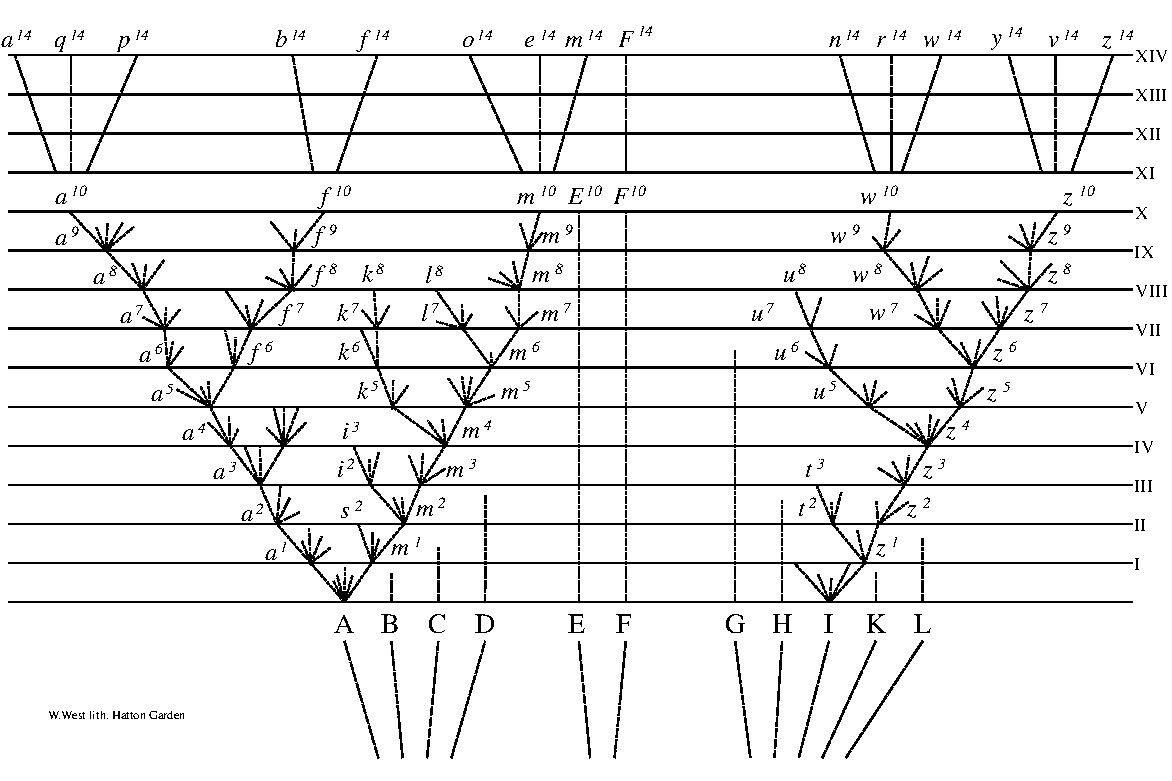
\includegraphics[width=0.7\textwidth]{../img/Origin_of_Species.pdf}
  \caption{«~Arbre de la vie~» de \nom{Darwin} (\emph{On the Origin of Species}, 1859). Les lettres représentent des espèces distinctes. Chaque ligne représente 1000 générations.}
  \label{fig:TreeOfLife}
\end{figure}

\begin{Definition}{L'arbre hiérarchique du Single-Linkage \cite{DendriteSingleLinkage1951, GowerRoss1969}}{single-linkage}
Étant donné un espace métrique fini $(\mathcal X, d)$ de $n$ points (dont on supposera les distances deux à deux distinctes), l'algorithme construit un dendrogramme (un arbre hiérarchique indexé par un niveau $r$) de la façon suivante :
\begin{itemize}
    \item \textbf{Initialisation} ($t=0$, niveau $r_0 \eqdef 0$). On part de la partition triviale en singletons, $\mathcal{C}^{r_0} \eqdef \bigl\{\{x_i\}\bigr\}_{i=1}^n$.
    \item \textbf{Itération} (étape $t$, niveau $r_t$). On fusionne les deux clusters $C$ et $C'$ présents dans le clustering $\mathcal{C}^{r_{t-1}}$ de l'étape précédente qui minimisent la distance de \emph{single linkage} :
    \[
        d_{\mathrm{SL}}(C, C') = \min_{x \in C, \, x' \in C'} d(x,x').
    \]
    On obtient alors un nouveau clustering $\mathcal{C}^{r_t}$ constitué de $n-t$ clusters associé au niveau $r_t \eqdef \tfrac12 d_{\mathrm{SL}}(C, C')$.
    \item \textbf{Arrêt}. L'algorithme se termine à l'étape $n-1$, lorsque tous les points sont réunis dans un unique cluster global (la racine de l'arbre) associé au niveau $r_{\mathrm{connect}} \eqdef r_{n-1}$.
\end{itemize}
\end{Definition}

\Remarque{Le Single-Linkage est souvent défini comme renvoyant une partition et non l'arbre hiérarchique complet. Dans sa version originale, il reçoit en effet $k$ le nombre de clusters à retourner et renvoie le clustering correspondant  à l'étape $n-k$. On peut aussi rencontrer le Single-Linkage dans sa version seuillée à $\varepsilon$ ; c'est-à-dire qu'il renvoie le clustering correspondant à l'étape $t \in \bigl\{ 0 ; \ldots ; n-1\bigr\}$, où $t$ est l'unique entier vérifiant $r_t \le \varepsilon < r_{t+1}$ (étant entendu, par convention, que $r_n \eqdef +\infty$).}

Cette définition incrémentale trouve un écho en théorie des graphes avec l'\emph{arbre minimum couvrant}. 



\section{Le Single-Linkage en pratique : l'arbre minimum couvrant}

\subsection{Différents algorithmes pour l'arbre minimum couvrant}

% L'équivalence algorithmique parfaite entre le Single-Linkage et l'arbre minimum couvrant (\emph{Minimum Spanning Tree}, MST) a été formellement prouvée par \textsc{Gower} \& \textsc{Ross} \cite{GowerRoss1969}. %Les fusions du premier dictent rigoureusement l'ordre d'insertion des arêtes du second sur le graphe complet de $\mathcal{X}$. 



%Pour extraire ce MST (parmi $\Theta(n^2)$ arêtes potentielles), trois paradigmes historiques s'affrontent, rigoureusement équivalents dans leur résultat final :

Il y a équivalence algorithmique entre le Single-Linkage et la recherche de l'arbre minimum couvrant (\emph{minimum spanning tree}, ou MST en anglais), comme l'illustre la version \nom{Borůvka} de construction de l'arbre minimum couvrant (voir ci-dessous). %a été formellement explicitée par \cite{GowerRoss1969} (bien que l'idée fût déjà implicite chez \cite{DendriteSingleLinkage1951}).

%(L'on pourrait d'ailleurs autoriser la fusion simultanée de plusieurs composantes, ce qui s'apparente conceptuellement à l'approche de l'algorithme de \nom{Borůvka}, voir \emph{infra}.)
%En effet, les fusions successives opérées par l'algorithme correspondent exactement à l'ajout progressif des arêtes par l'algorithme de \nom{Borůvka} (ou de \nom{Kruskal}). En supprimant les $m-1$ arêtes les plus longues de l'arbre minimum couvrant, on retrouve la partition exacte en $m$ clusters du Single-Linkage.

Il existe trois algorithmes historiques pour extraire l'arbre minimum couvrant d'un graphe (connexe) à $n$ nœuds et $m$ arêtes.

\begin{itemize}
    \item \textbf{``Single-Linkage parallèle'' : \textsc{Borůvka}} (1926) \cite{Boruvka1926}. À chaque itération, chaque composante connexe identifie et contracte son arête sortante la plus courte. Le nombre de composantes diminue de moitié à chaque passe, garantissant une complexité en $\mathcal{O}(m \log n)$. Il s'agit d'un Single-Linkage massivement parallélisé.

    \item \textbf{Approche gloutonne : \textsc{Kruskal}} (1956) \cite{Kruskal1956}. Les arêtes sont triées par poids croissant, puis insérées séquentiellement sous réserve de ne former aucun cycle\footnote{Rappelons qu'un arbre est par définition un graphe connexe acyclique.}. L'étape limitante est le tri des arêtes, de complexité $\mathcal{O}(\operatorname{Tri}(m))$ (citons le \texttt{QuickSort} \cite{Hoare1962} en complexité moyenne $\mathcal O (m \log m)$ de \textsc{Hoare}\footnote{Tony \textsc{Hoare} (1934 -- †2026), décédé alors que j'allais me lancer dans rédaction de ce manuscrit.}). C'est en pratique la méthode la plus utilisée, tant pour sa simplicité que pour la complexité mémoire optimale en $\mathcal{O}(n)$ de la structure auxiliaire d'ensembles disjoints (\texttt{Union-Find}) \cite{Tarjan1975} utilisée une fois le tri des arêtes effectué.

    \item \textbf{Croissance locale : \textsc{Jarník}--\textsc{Prim}--\textsc{Dijkstra}} (1930/1957/1959). Cet algorithme fait croître un \emph{unique} arbre en y rattachant itérativement le sommet non visité le plus proche. Sur un espace géométrique dense, son exécution en $\mathcal{O}(n^2)$ est asymptotiquement optimale.
\end{itemize}

\paragraph{Améliorations (théoriques) et avancée récente}
%L'algorithme par contraction d'arêtes de \nom{Borůvka} offre une excellente complexité en $\mathcal{O}(m \log n)$ pour les graphes peu denses 
Il existe des raffinements théoriques pour améliorer le facteur $\log n$ de la complexité \cite{ChazelleMST}. Il a d'ailleurs été montré que la complexité optimale, quoique non calculée explicitement, est celle associée à un certain arbre de décision (\emph{decision tree}) \cite{OptimalMST2002}.
Il existe aussi des algorithmes aléatoires pour retrouver l'arbre minimum couvrant \cite{RandomizedMST}. 
Citons enfin une avancée récente en intelligence artificielle dans le cas d'espaces métriques : \nom{Veldt} \emph{et al.} \cite{Veldt2025} ont présenté un algorithme de complétion de forêts par apprentissage (\emph{learning-augmented algorithms}) en temps sous-quadratique (esquivant ainsi le parcours exhaustif de la matrice des distances).



\subsection{Graphe de \textsc{Gabriel} et triangulation de \textsc{Delaunay}}

\paragraph{Le cas de la basse dimension euclidienne ($p=2, 3, 4 , \ldots$)}
Dans le cas particulier où les données $\mathcal X \subset \mathbb R^p$ sont dans l'espace euclidien, on peut exploiter la géométrie de cet espace et restreindre la recherche de l'arbre minimum couvrant à des graphes géométriques beaucoup plus parcimonieux que le graphe complet. Ces méthodes sont particulièrement efficaces lorsque la dimension $p$ est suffisamment faible (\emph{cf.} par exemple la discussion \emph{infra} dans le cas du plan $p=2$).

Les arêtes de ces graphes reposent sur une condition de vacuité d'une région entre les deux sommets (voir \Fig~\ref{fig:Gabriel_RelativeNeighbourhood} pour une illustration).

\begin{Definition}{Graphe de voisinage relatif \cite{Toussaint1980}}{rng}
Le graphe de voisinage relatif (\emph{relative neighborhood graph}, ou RNG en anglais) relie deux points $x, x' \in \mathcal X$ si l'intersection de leurs boules ouvertes de rayon $\norme{x-x'}$ est vide de tout point de $\mathcal X$ :
\[
    \forall z \in \mathcal X \setminus \{x,x'\}, \quad \max \bigl( \norme{x-z}, \norme{x'-z} \bigr) \ge \norme{x-x'}.
\]
\end{Definition}

\begin{Definition}{Graphe de \nom{Gabriel} \cite{GabrielSokal1969}}{gabriel}
Le graphe de \nom{Gabriel} relie deux points $x, x' \in \mathcal X$ si la boule ouverte de diamètre $[x,x']$ ne contient aucun point de $\mathcal X$ :
\[
    \forall z \in \mathcal X \setminus \{x,x'\}, \quad \norme{x-z}^2 + \norme{x'-z}^2 \ge \norme{x-x'}^2.
\]
\end{Definition}

\begin{Definition}{Triangulation de \nom{Delaunay} \cite{Delaunay1934, BoissonnatChazalYvinec}}{delaunay}
Le graphe de \nom{Delaunay} (le $1$-squelette de la triangulation de \nom{Delaunay}) relie deux points $x, x' \in \mathcal X$ s'il existe au moins une boule ouverte, vide de tout point de $\mathcal X$, dont la frontière contient simultanément $x$ et $x'$.
\end{Definition}

\begin{figure}[!ht]
    \centering
    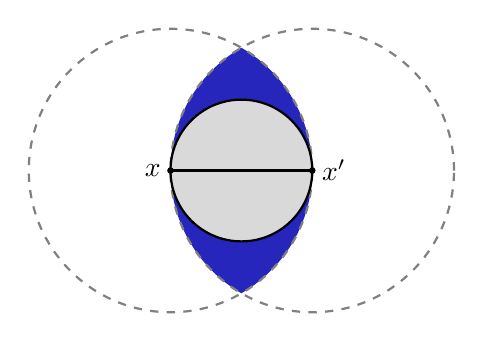
\begin{tikzpicture}[scale=0.6]
        \coordinate (x) at (0,0);
        \coordinate (xp) at (3,0);
        \coordinate (M) at (1.5,0);
        
        % Voisinage relatif (lune d'intersection)
        \begin{scope}
            \clip (x) circle (3);
            \fill[blue!70!black, fill opacity=0.85] (xp) circle (3);
        \end{scope}
        
        % Graphe de Gabriel (disque diamétral)
        \fill[black!15] (M) circle (1.5);
        
        \draw[thick, dashed, gray] (x) circle (3);
        \draw[thick, dashed, gray] (xp) circle (3);
        \draw[thick] (M) circle (1.5);
        
        \fill (x) circle (2pt) node[left] {$x$};
        \fill (xp) circle (2pt) node[right] {$x'$};
        \draw[thick] (x) -- (xp);
    \end{tikzpicture}
    \caption{L'arête $(x,x')$ appartient au graphe de \textcolor{gray}{\textbf{\textsc{Gabriel}}} si aucun autre point de $\mathcal{X}$ ne tombe dans le disque de diamètre $[x,x']$ (en gris). Elle appartient au graphe de voisinage relatif (\emph{relative neighborhood graph}, \textcolor{blue!70!black}{\textbf{RNG}}) si aucun point ne tombe dans l'intersection des deux disques de rayon $\protect\norme{x-x'}$ centrés en $x$ et $x'$ (en bleu foncé).}
    \label{fig:Gabriel_RelativeNeighbourhood}
\end{figure}

\begin{Resultat}{L'arbre minimum couvrant (euclidien) est un sous-graphe de graphes géométriques \cite{BoissonnatChazalYvinec}}{MSTsous-graphe}
L'arbre minimum couvrant euclidien est un sous-graphe du graphe de voisinage relatif ({RNG}), lui-même inclus dans le graphe de \nom{Gabriel}, qui est à son tour un sous-graphe de la triangulation de \nom{Delaunay} \cite{BoissonnatChazalYvinec} :
\[
    \mathrm{MST} \ \subseteq \ \mathrm{RNG} \ \subseteq \ \text{\textsc{Gabriel}} \ \subseteq \ \text{\textsc{Delaunay}}.
\]
\end{Resultat}

\paragraph{Le cas du plan $p=2$}
Dans le plan $\mathbb R^2$, la triangulation de \nom{Delaunay} possède un nombre d'arêtes linéaire (au plus $3n-6$) et se calcule en $\mathcal{O}(n \log n)$ \cite{BoissonnatChazalYvinec}. L'algorithme du Single-Linkage hérite par conséquent de cette même complexité.

\section{Le Single-Linkage en théorie : persistance de graphes géométriques}

Une autre façon très féconde d'aborder le Single-Linkage est de le voir comme un processus d'\emph{analyse persistante} (terme forgé par analogie avec l'\emph{homologie persistante} \cite{BobrowskiKahle}), consistant à observer la naissance et la fusion de composantes lorsque l'on fait varier un paramètre d'échelle $r$.

\begin{Definition}{Graphe géométrique (au sens de \nom{Gilbert}-\nom{Penrose} \cite{Gilbert1961, penrose2003})}{gg}
Soit $(\mathcal X, d)$ un espace métrique. Étant donné un rayon $r \ge 0$, le graphe géométrique $\mathcal{G}(\mathcal{X}, r)$ est le graphe dont les sommets sont les points $\mathcal{X}$, et où deux points $x, x' \in \mathcal{X}$ sont reliés par une arête si et seulement si \[
\norme{x - x'} \le 2r.
\]
\end{Definition}

L'équivalence fondamentale entre l'arbre minimum couvrant et l'évolution des graphes géométriques s'énonce avec le joli résultat suivant (\Res~\ref{res:chapIV_mst_sous_niveaux_graphe} \& son corollaire, le \Th~\ref{th:mst_gg}) qui, quoique fondamental, n'est que très rarement explicitement mentionné ; \nom{Penrose} \cite{penrose2003} l'utilise implicitement. 
L'on est contraint d'adopter le formalisme de l'analyse topologique de données (\emph{topological data analysis}, TDA) pour le voir écrit noir sur blanc (voir \cite{DeyWang2022}, Theorem 3.18 et la remarque « Connection to minimum spanning tree »).


% \textcolor{red}{Plutôt que le théorème ci-après, insérer le résultat suivant :}

%Le résultat général sur lequel repose tout arbre couvrant minimum est le suivant.

\begin{Resultat}{Arbre minimum couvrant et sous-niveaux d'un graphe pondéré \cite{Kruskal1956, Prim1957}}{chapIV_mst_sous_niveaux_graphe}
Soit $G=(V,E,w)$ un graphe fini pondéré, et soit $T$ une forêt minimum couvrante de $G$ (un arbre minimum couvrant si $G$ est connexe). Alors, pour tout $r\ge0$, les composantes connexes de
\[
    T_{\le r}=(V,\{e\in T:w(e)\le r\})
\]
sont exactement les mêmes que celles de
\[
    G_{\le r}=(V,\{e\in E:w(e)\le r\}).
\]
\end{Resultat}
\Remarque{Par abus de langage, nous parlons de ``composante connexe'' pour désigner l'ensemble des nœuds du sous-graphe induit (et non le sous-graphe lui-même).}

\begin{Preuve}[Preuve du \Res~\ref{res:chapIV_mst_sous_niveaux_graphe}]
Soir $r \ge 0$. L'inclusion $T_{\le r}\subseteq G_{\le r}$ est immédiate. Pour l'autre sens, supposons que deux sommets $u,v$ soient connectés dans $G_{\le r}$ mais pas dans $T_{\le r}$. Sur l'unique chemin de $T$ reliant $u$ à $v$, il existe donc une arête $e$ de poids strictement supérieur à $r$. Retirer $e$ de $T$ définit une coupe $(A,V\setminus A)$. Comme $u$ et $v$ sont connectés dans $G_{\le r}$, il existe une arête $e'$ de $G_{\le r}$ qui traverse cette coupe (voir le \Res~\ref{res:prim} ci-après). Alors
\[
    w(e')\le r < w(e),
\]
et remplacer $e$ par $e'$ donnerait une forêt couvrante de poids strictement plus petit, en contradiction avec la minimalité de $T$.
\end{Preuve}


\begin{Resultat}{Coupe et arbre minimum couvrant \cite{Prim1957}}{prim}
En reprenant les notations du \Res~\ref{res:chapIV_mst_sous_niveaux_graphe}, soit
 $V =  V_1 \UnionDisjointe V_2$ une partition de l'ensemble des sommets, alors il existe une arête $e \in E$ de poids minimum reliant $V_1$ à $V_2$ qui soit aussi dans $T$.
\end{Resultat}
% \begin{Resultat}{Les sous-arbres d'un arbre minimum couvrant sont encore des arbres minimums couvrants}{sous_arbres}
% Retirer une arête de l'arbre minimum couvrant scinde celui-ci en deux composantes, qui s'avèrent être les arbres minimums couvrants de leurs sommets respectifs.
% \end{Resultat}

% \begin{Preuve}[\textsc{Preuve du Théorème~\ref{th:mst_gg}}]
% Le résultat est trivial pour $n=1$. Supposons $n \ge 2$.
% Pour tout $r \ge 0$, on a l'inclusion $\mathrm{MST}_{\le r} \subseteq \mathcal{G}(\mathcal{X}, r)$ (toute arête conservée dans l'arbre a une longueur $\le 2r$). 

% Pour montrer l'inclusion réciproque au niveau des composantes, procédons par récurrence sur $n$. Définissons $r_{\mathrm{connect}}$ comme le seuil critique à partir duquel $\mathcal{G}(\mathcal{X}, r)$ devient connexe. 
% Pour $r \ge r_{\mathrm{connect}}$, $\mathcal{G}(\mathcal{X}, r)$ est connexe. Pour toute partition $\mathcal X = \mathcal X_1 \UnionDisjointe \mathcal X_2$, il existe une arête de taille $\le 2r$ la traversant. D'après le \Res~\ref{res:prim}, une telle arête (ou une plus courte) est dans le $\mathrm{MST}$. 
% La partition ayant été choisie arbitrairement, $\mathrm{MST}_{\le r}$ est également connexe.

% Si l'on prend un rayon $r < r_{\mathrm{connect}}$ suffisamment proche du seuil de sorte que seule l'arête la plus longue de $\mathcal{G}(\mathcal{X}, r_{\mathrm{connect}})$ ait disparu, le graphe géométrique se scinde en deux composantes connexes $\mathcal{X}_1$ et $\mathcal{X}_2$ (voir \Fig~\ref{fig:r_connect}). Parallèlement, supprimer cette arête de l'arbre global (qui en est nécessairement la plus longue) le scinde en deux composantes, qui ont nécessairement pour sommets $\mathcal{X}_1$ et $\mathcal{X}_2$. En appliquant l'hypothèse de récurrence sur les sous-arbres induits par le \Res~\ref{res:sous_arbres}, la correspondance des composantes connexes est prouvée pour tout $r$.
% \end{Preuve}

Le \Th~\ref{th:mst_gg} suivant est un corollaire du \Res~\ref{res:chapIV_mst_sous_niveaux_graphe}.

\begin{Theoreme}{Graphe géométrique $\equiv$ Arbre minimum couvrant élagué}{mst_gg}
(Pour avoir l'unicité de l'arbre minimum couvrant, l'on suppose que les points de $\mathcal X$ sont en position générale.) 
Pour tout rayon $r \ge 0$, les ensembles de sommets des composantes connexes de l'arbre minimum couvrant élagué de ses arêtes de longueur strictement supérieure à $2r$ (noté $\mathrm{MST}_{\le r}$) coïncident exactement avec ceux du graphe géométrique $\mathcal{G}(\mathcal{X}, r)$.
\end{Theoreme}
\Remarque{Pour un graphe sur $\mathcal X \subset \mathbb R^p$, avoir ses sommets \emph{en posisition générale} signifie que les distances entre paires de points sont distinctes deux à deux, assurant l'unicité de l'arbre minimum couvrant. Nous reviendrons plus tard sur la notion de \emph{position générale} pour un nuage de points lorsqu'il s'agira de généraliser aux hypergraphes (voir \Def[def:chapIV_position_generale_cech]).}

Le \Th~\ref{th:mst_gg} est illustré avec la \Fig~\ref{fig:MST_GrapheGeometrique}.

\begin{figure}[!ht]
  \centering
  \begin{subfigure}[b]{0.43\textwidth}
  \resizebox{\linewidth}{!}{
  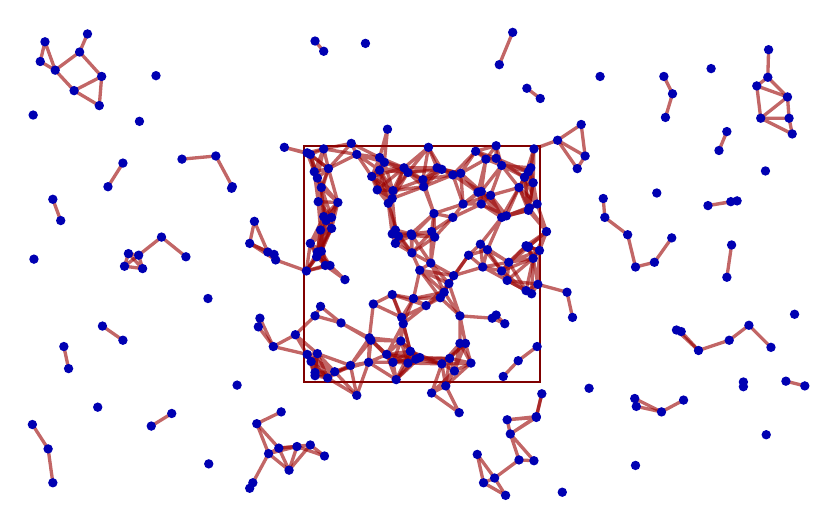
\begin{tikzpicture}[>=stealth]
    \tikzset{dot/.style={circle, fill=blue!70!black, inner sep=1.2pt, outer sep=0pt}}
    \tikzset{edge/.style={line width=1.2pt, red!60!black, opacity=0.6}}
    \tikzset{sq/.style={thick, red!50!black}}

    \draw[sq] (3.5, 1.5) rectangle (6.5, 4.5);
      \draw[edge] (3.75,5.70)--(3.64,5.83) (7.32,3.59)--(7.30,3.83) (7.32,3.59)--(7.61,3.37) (1.56,0.94)--(1.82,1.10) (0.58,5.20)--(0.34,5.46) (0.58,5.20)--(0.90,5.01) (0.58,5.20)--(0.93,5.38) (6.01,4.25)--(5.68,4.43) (6.01,4.25)--(6.38,4.22) (6.01,4.25)--(5.75,3.92) (6.01,4.25)--(5.87,3.87) (6.01,4.25)--(5.94,4.34) (6.01,4.25)--(6.35,4.17) (6.01,4.25)--(6.23,3.97) (6.01,4.25)--(6.30,4.10) (6.01,4.25)--(5.94,4.50) (6.01,4.25)--(5.81,4.33) (0.21,5.82)--(0.34,5.46) (0.21,5.82)--(0.15,5.57) (8.32,1.27)--(8.04,1.12) (3.04,3.15)--(3.12,3.12) (3.04,3.15)--(2.81,3.26) (3.04,3.15)--(3.14,3.05) (3.04,3.15)--(2.87,3.54) (4.32,1.75)--(3.89,1.63) (4.32,1.75)--(4.17,1.33) (4.32,1.75)--(4.09,1.71) (4.32,1.75)--(4.35,2.03) (4.32,1.75)--(4.67,1.53) (4.32,1.75)--(4.55,1.85) (4.32,1.75)--(4.63,1.75) (4.32,1.75)--(4.33,2.06) (6.12,0.84)--(6.08,1.02) (6.12,0.84)--(6.45,1.05) (6.12,0.84)--(6.42,0.50) (6.12,0.84)--(6.45,1.06) (6.12,0.84)--(6.23,0.51) (2.92,2.20)--(3.11,1.95) (2.92,2.20)--(2.94,2.31) (4.56,4.71)--(4.52,4.29) (4.56,4.71)--(4.46,4.35) (2.00,3.09)--(1.69,3.34) (5.92,0.28)--(6.06,0.06) (5.92,0.28)--(5.70,0.58) (5.92,0.28)--(5.78,0.22) (5.92,0.28)--(6.23,0.51) (6.08,1.02)--(6.45,1.05) (6.08,1.02)--(6.45,1.06) (0.65,5.69)--(0.34,5.46) (0.65,5.69)--(0.75,5.92);
      \draw[edge] (0.65,5.69)--(0.93,5.38) (9.66,4.85)--(9.70,4.65) (9.66,4.85)--(9.30,4.85) (9.66,4.85)--(9.64,5.12) (3.05,0.59)--(3.31,0.38) (3.05,0.59)--(2.90,0.97) (3.05,0.59)--(3.18,0.66) (3.05,0.59)--(2.85,0.22) (3.05,0.59)--(3.41,0.68) (6.84,2.64)--(6.91,2.32) (6.84,2.64)--(6.47,2.74) (1.22,2.97)--(1.45,2.94) (1.22,2.97)--(1.40,3.11) (1.22,2.97)--(1.27,3.13) (0.34,5.46)--(0.15,5.57) (2.59,3.98)--(2.38,4.37) (2.59,3.98)--(2.58,3.96) (3.12,3.12)--(2.81,3.26) (3.12,3.12)--(3.14,3.05) (5.47,1.11)--(5.12,1.36) (5.47,1.11)--(5.30,1.45) (9.70,4.65)--(9.30,4.85) (9.39,5.37)--(9.25,5.26) (9.39,5.37)--(9.40,5.72) (9.39,5.37)--(9.64,5.12) (5.98,5.53)--(6.15,5.94) (0.45,1.95)--(0.51,1.67) (3.89,1.63)--(4.17,1.33) (3.89,1.63)--(3.59,1.76) (3.89,1.63)--(3.54,1.85) (3.89,1.63)--(3.64,1.62) (3.89,1.63)--(4.09,1.71) (3.89,1.63)--(3.80,1.55) (3.89,1.63)--(3.67,1.86) (3.89,1.63)--(3.64,1.58) (8.29,2.14)--(8.51,1.90) (8.29,2.14)--(8.23,2.16) (2.81,3.26)--(3.14,3.05) (2.81,3.26)--(2.87,3.54) (7.72,1.19)--(8.04,1.12) (7.72,1.19)--(7.70,1.29) (7.07,4.37)--(6.72,4.57) (7.07,4.37)--(6.97,4.21) (7.07,4.37)--(7.02,4.77) (3.58,0.70)--(3.31,0.38) (3.58,0.70)--(3.18,0.66) (3.58,0.70)--(3.41,0.68) (3.58,0.70)--(3.76,0.56) (8.63,3.74)--(9.00,3.80) (8.63,3.74)--(8.92,3.79);
      \draw[edge] (3.31,0.38)--(3.18,0.66) (3.31,0.38)--(3.41,0.68) (3.11,1.95)--(3.39,2.10) (3.11,1.95)--(2.94,2.31) (3.11,1.95)--(3.54,1.85) (8.87,2.83)--(8.93,3.24) (1.20,4.28)--(1.01,3.98) (7.61,3.37)--(7.71,2.96) (7.71,2.96)--(7.95,3.02) (5.23,2.57)--(5.05,2.47) (5.23,2.57)--(5.48,2.34) (5.23,2.57)--(4.97,2.92) (5.23,2.57)--(5.40,2.85) (5.23,2.57)--(4.89,2.56) (5.23,2.57)--(5.34,2.75) (5.23,2.57)--(5.28,2.64) (0.25,0.65)--(0.05,0.96) (0.25,0.65)--(0.31,0.22) (0.31,3.82)--(0.41,3.55) (3.14,3.05)--(3.53,2.91) (9.08,1.50)--(9.08,1.44) (4.10,4.53)--(3.81,4.21) (4.10,4.53)--(4.46,4.35) (4.10,4.53)--(3.75,4.46) (4.10,4.53)--(4.17,4.39) (2.90,0.97)--(3.18,0.66) (2.90,0.97)--(3.21,1.12) (9.30,4.85)--(9.25,5.26) (9.30,4.85)--(9.64,5.12) (6.33,5.23)--(6.50,5.10) (8.04,1.12)--(7.70,1.29) (8.07,5.38)--(8.18,5.16) (3.18,0.66)--(3.41,0.68) (8.18,5.16)--(8.09,4.86) (4.17,1.33)--(4.09,1.71) (4.17,1.33)--(3.80,1.55) (1.20,2.03)--(0.94,2.21) (9.43,1.94)--(9.15,2.22) (5.19,4.22)--(5.49,4.15) (5.19,4.22)--(5.01,4.07) (5.19,4.22)--(5.39,4.13) (5.19,4.22)--(5.02,3.98) (5.19,4.22)--(4.82,4.16) (5.19,4.22)--(4.77,4.22) (5.19,4.22)--(5.08,4.48) (5.19,4.22)--(5.25,4.20) (9.62,1.51)--(9.86,1.45) (4.97,1.81)--(4.82,1.74) (4.97,1.81)--(4.73,2.02) (4.97,1.81)--(4.92,1.79);
      \draw[edge] (4.97,1.81)--(4.67,1.53) (4.97,1.81)--(4.55,1.85) (4.97,1.81)--(5.35,1.80) (4.97,1.81)--(4.63,1.75) (4.97,1.81)--(5.25,1.73) (4.97,1.81)--(4.85,1.89) (2.85,0.22)--(2.81,0.15) (6.10,3.02)--(6.34,3.21) (6.10,3.02)--(5.77,2.96) (6.10,3.02)--(6.32,3.23) (6.10,3.02)--(6.32,2.66) (6.10,3.02)--(6.08,2.79) (6.10,3.02)--(6.35,3.22) (6.10,3.02)--(5.83,3.18) (6.10,3.02)--(5.74,3.25) (6.10,3.02)--(6.41,3.07) (6.10,3.02)--(6.01,2.91) (6.10,3.02)--(6.49,3.17) (1.45,2.94)--(1.40,3.11) (1.45,2.94)--(1.27,3.13) (6.72,4.57)--(6.97,4.21) (6.72,4.57)--(7.02,4.77) (6.72,4.57)--(6.42,4.46) (2.38,4.37)--(1.95,4.33) (3.68,3.79)--(3.71,3.43) (3.68,3.79)--(3.78,3.55) (3.68,3.79)--(3.85,3.59) (3.68,3.79)--(3.81,4.21) (3.68,3.79)--(3.93,3.78) (3.68,3.79)--(3.75,3.60) (3.68,3.79)--(3.72,3.97) (3.68,3.79)--(3.85,3.45) (3.68,3.79)--(3.63,4.17) (3.68,3.79)--(3.67,4.09) (6.34,3.21)--(6.58,3.41) (6.34,3.21)--(6.32,3.23) (6.34,3.21)--(6.35,3.22) (6.34,3.21)--(6.41,3.07) (6.34,3.21)--(6.01,2.91) (6.34,3.21)--(6.49,3.17) (0.90,5.01)--(0.93,5.38) (5.12,1.36)--(5.30,1.45) (5.12,1.36)--(5.41,1.64) (5.12,1.36)--(5.25,1.73) (6.45,1.05)--(6.52,1.35) (6.45,1.05)--(6.45,1.06) (3.41,0.68)--(3.76,0.56) (9.25,5.26)--(9.64,5.12) (8.17,3.33)--(7.95,3.02) (5.30,1.45)--(5.41,1.64);
      \draw[edge] (5.30,1.45)--(5.35,1.80) (5.30,1.45)--(5.62,1.74) (5.30,1.45)--(5.25,1.73) (9.00,3.80)--(8.92,3.79) (3.39,2.10)--(3.59,1.76) (3.39,2.10)--(3.54,1.85) (3.39,2.10)--(3.67,1.86) (3.39,2.10)--(3.64,2.34) (8.87,4.68)--(8.77,4.44) (6.42,0.50)--(6.23,0.51) (6.06,0.06)--(5.78,0.22) (5.49,4.15)--(5.68,4.43) (5.49,4.15)--(5.39,4.13) (5.49,4.15)--(5.71,3.91) (5.49,4.15)--(5.75,3.92) (5.49,4.15)--(5.52,3.76) (5.49,4.15)--(5.25,4.20) (5.49,4.15)--(5.81,4.33) (6.52,1.35)--(6.45,1.06) (3.25,4.48)--(3.58,4.39) (3.25,4.48)--(3.54,4.41) (6.58,3.41)--(6.36,3.71) (6.58,3.41)--(6.32,3.23) (6.58,3.41)--(6.35,3.22) (6.58,3.41)--(6.46,3.76) (6.58,3.41)--(6.41,3.07) (6.58,3.41)--(6.35,3.68) (6.58,3.41)--(6.49,3.17) (5.77,2.96)--(6.08,2.79) (5.77,2.96)--(5.40,2.85) (5.77,2.96)--(5.83,3.18) (5.77,2.96)--(5.74,3.25) (5.77,2.96)--(5.59,3.11) (5.77,2.96)--(6.01,2.91) (9.15,2.22)--(8.90,2.03) (8.51,1.90)--(8.90,2.03) (8.51,1.90)--(8.23,2.16) (1.69,3.34)--(1.40,3.11) (5.70,0.58)--(5.78,0.22) (1.40,3.11)--(1.27,3.13) (3.59,1.76)--(3.54,1.85) (3.59,1.76)--(3.64,1.62) (3.59,1.76)--(3.80,1.55) (3.59,1.76)--(3.67,1.86) (3.59,1.76)--(3.64,1.58) (5.11,3.01)--(5.12,3.41) (5.11,3.01)--(5.16,3.34) (5.11,3.01)--(4.97,2.92) (5.11,3.01)--(4.87,3.14) (5.11,3.01)--(5.40,2.85);
      \draw[edge] (5.11,3.01)--(4.86,3.38) (5.11,3.01)--(4.87,3.36) (5.11,3.01)--(5.34,2.75) (5.11,3.01)--(5.28,2.64) (4.66,3.26)--(4.70,3.35) (4.66,3.26)--(4.62,3.38) (4.66,3.26)--(4.66,3.43) (4.66,3.26)--(4.87,3.14) (4.66,3.26)--(4.86,3.38) (4.66,3.26)--(4.87,3.36) (3.66,3.09)--(3.71,3.43) (3.66,3.09)--(3.58,3.26) (3.66,3.09)--(3.77,2.98) (3.66,3.09)--(3.67,3.15) (3.66,3.09)--(3.83,2.98) (3.66,3.09)--(3.53,2.91) (3.66,3.09)--(3.85,3.45) (3.66,3.09)--(3.72,3.16) (5.12,3.41)--(5.15,3.64) (5.12,3.41)--(5.16,3.34) (5.12,3.41)--(4.70,3.35) (5.12,3.41)--(4.87,3.14) (5.12,3.41)--(5.39,3.59) (5.12,3.41)--(4.86,3.38) (5.12,3.41)--(4.87,3.36) (5.68,4.43)--(5.39,4.13) (5.68,4.43)--(5.94,4.34) (5.68,4.43)--(5.94,4.50) (5.68,4.43)--(5.81,4.33) (5.05,2.47)--(4.76,2.24) (5.05,2.47)--(4.62,2.61) (5.05,2.47)--(4.89,2.56) (5.05,2.47)--(5.34,2.75) (5.05,2.47)--(5.28,2.64) (5.05,2.47)--(4.74,2.32) (5.89,2.31)--(5.48,2.34) (5.89,2.31)--(5.94,2.35) (5.89,2.31)--(6.05,2.24) (4.82,1.74)--(4.73,2.02) (4.82,1.74)--(4.92,1.79) (4.82,1.74)--(4.67,1.53) (4.82,1.74)--(4.55,1.85) (4.82,1.74)--(4.63,1.75) (4.82,1.74)--(5.25,1.73) (4.82,1.74)--(4.85,1.89) (3.58,4.39)--(3.81,4.21) (3.58,4.39)--(3.72,3.97) (3.58,4.39)--(3.75,4.46) (3.58,4.39)--(3.54,4.41) (3.58,4.39)--(3.63,4.17);
      \draw[edge] (3.58,4.39)--(3.67,4.09) (6.01,3.59)--(6.36,3.71) (6.01,3.59)--(6.07,3.61) (6.01,3.59)--(5.71,3.91) (6.01,3.59)--(5.75,3.92) (6.01,3.59)--(5.75,3.76) (6.01,3.59)--(5.87,3.87) (6.01,3.59)--(5.83,3.18) (6.01,3.59)--(5.74,3.25) (6.01,3.59)--(6.23,3.97) (6.01,3.59)--(6.35,3.68) (4.73,2.02)--(4.76,2.24) (4.73,2.02)--(4.92,1.79) (4.73,2.02)--(4.35,2.03) (4.73,2.02)--(4.55,1.85) (4.73,2.02)--(4.63,1.75) (4.73,2.02)--(4.33,2.06) (4.73,2.02)--(4.74,2.32) (4.73,2.02)--(4.85,1.89) (3.97,2.25)--(3.71,2.46) (3.97,2.25)--(4.35,2.03) (3.97,2.25)--(3.64,2.34) (3.97,2.25)--(4.33,2.06) (5.15,3.64)--(5.16,3.34) (5.15,3.64)--(5.01,4.07) (5.15,3.64)--(5.02,3.98) (5.15,3.64)--(5.52,3.76) (5.15,3.64)--(5.39,3.59) (5.15,3.64)--(4.86,3.38) (5.15,3.64)--(4.87,3.36) (5.48,2.34)--(5.48,1.99) (5.48,2.34)--(5.55,1.99) (5.48,2.34)--(5.34,2.75) (5.48,2.34)--(5.28,2.64) (6.36,3.71)--(6.07,3.61) (6.36,3.71)--(6.46,3.76) (6.36,3.71)--(6.23,3.97) (6.36,3.71)--(6.35,3.68) (6.36,3.71)--(6.30,4.10) (6.36,3.71)--(6.41,4.03) (5.16,3.34)--(4.87,3.14) (5.16,3.34)--(5.39,3.59) (5.16,3.34)--(4.86,3.38) (5.16,3.34)--(4.87,3.36) (4.76,2.24)--(4.55,1.85) (4.76,2.24)--(4.62,2.61) (4.76,2.24)--(4.89,2.56) (4.76,2.24)--(4.74,2.32) (4.76,2.24)--(4.85,1.89) (4.57,3.77)--(4.70,3.35);
      \draw[edge] (4.57,3.77)--(4.62,3.38) (4.57,3.77)--(4.66,3.43) (4.57,3.77)--(4.62,3.83) (4.57,3.77)--(4.46,4.19) (4.57,3.77)--(4.36,4.11) (4.57,3.77)--(4.43,3.94) (4.57,3.77)--(4.63,3.93) (3.54,1.85)--(3.64,1.62) (3.54,1.85)--(3.80,1.55) (3.54,1.85)--(3.67,1.86) (3.54,1.85)--(3.64,1.58) (3.64,1.62)--(3.80,1.55) (3.64,1.62)--(3.67,1.86) (3.64,1.62)--(3.64,1.58) (6.07,3.61)--(5.75,3.92) (6.07,3.61)--(5.75,3.76) (6.07,3.61)--(5.87,3.87) (6.07,3.61)--(6.46,3.76) (6.07,3.61)--(6.23,3.97) (6.07,3.61)--(6.35,3.68) (4.92,1.79)--(4.67,1.53) (4.92,1.79)--(4.55,1.85) (4.92,1.79)--(5.35,1.80) (4.92,1.79)--(4.63,1.75) (4.92,1.79)--(5.25,1.73) (4.92,1.79)--(4.85,1.89) (4.97,2.92)--(4.87,3.14) (4.97,2.92)--(5.40,2.85) (4.97,2.92)--(4.89,2.56) (4.97,2.92)--(5.34,2.75) (4.97,2.92)--(5.28,2.64) (4.02,2.80)--(3.77,2.98) (4.02,2.80)--(3.83,2.98) (4.70,3.35)--(4.62,3.38) (4.70,3.35)--(4.66,3.43) (4.70,3.35)--(4.87,3.14) (4.70,3.35)--(4.86,3.38) (4.70,3.35)--(4.87,3.36) (5.41,1.64)--(5.48,1.99) (5.41,1.64)--(5.35,1.80) (5.41,1.64)--(5.62,1.74) (5.41,1.64)--(5.25,1.73) (5.41,1.64)--(5.55,1.99) (4.62,3.38)--(4.66,3.43) (4.62,3.38)--(4.87,3.14) (4.62,3.38)--(4.86,3.38) (4.62,3.38)--(4.87,3.36) (5.01,4.07)--(5.39,4.13) (5.01,4.07)--(5.02,3.98) (5.01,4.07)--(4.82,4.16);
      \draw[edge] (5.01,4.07)--(4.77,4.22) (5.01,4.07)--(5.08,4.48) (5.01,4.07)--(5.25,4.20) (5.01,4.07)--(4.63,3.93) (5.48,1.99)--(5.35,1.80) (5.48,1.99)--(5.62,1.74) (5.48,1.99)--(5.25,1.73) (5.48,1.99)--(5.55,1.99) (3.71,3.43)--(3.58,3.26) (3.71,3.43)--(3.78,3.55) (3.71,3.43)--(3.85,3.59) (3.71,3.43)--(3.77,2.98) (3.71,3.43)--(3.67,3.15) (3.71,3.43)--(3.93,3.78) (3.71,3.43)--(3.75,3.60) (3.71,3.43)--(3.85,3.45) (3.71,3.43)--(3.72,3.16) (3.58,3.26)--(3.78,3.55) (3.58,3.26)--(3.85,3.59) (3.58,3.26)--(3.77,2.98) (3.58,3.26)--(3.67,3.15) (3.58,3.26)--(3.75,3.60) (3.58,3.26)--(3.83,2.98) (3.58,3.26)--(3.53,2.91) (3.58,3.26)--(3.85,3.45) (3.58,3.26)--(3.72,3.16) (6.32,3.23)--(6.35,3.22) (6.32,3.23)--(6.41,3.07) (6.32,3.23)--(6.01,2.91) (6.32,3.23)--(6.49,3.17) (4.66,3.43)--(4.87,3.14) (4.66,3.43)--(4.62,3.83) (4.66,3.43)--(4.86,3.38) (4.66,3.43)--(4.87,3.36) (4.87,3.14)--(4.86,3.38) (4.87,3.14)--(4.87,3.36) (6.32,2.66)--(6.47,2.74) (6.32,2.66)--(6.08,2.79) (6.32,2.66)--(6.39,2.62) (6.32,2.66)--(6.41,3.07) (6.32,2.66)--(6.01,2.91) (6.38,4.22)--(6.35,4.17) (6.38,4.22)--(6.42,4.46) (6.38,4.22)--(6.23,3.97) (6.38,4.22)--(6.30,4.10) (6.38,4.22)--(6.41,4.03) (4.09,1.71)--(3.80,1.55) (4.09,1.71)--(4.35,2.03) (4.09,1.71)--(3.67,1.86) (4.09,1.71)--(4.33,2.06);
      \draw[edge] (3.80,1.55)--(3.67,1.86) (3.80,1.55)--(3.64,1.58) (3.78,3.55)--(3.85,3.59) (3.78,3.55)--(3.67,3.15) (3.78,3.55)--(3.93,3.78) (3.78,3.55)--(3.75,3.60) (3.78,3.55)--(3.72,3.97) (3.78,3.55)--(3.85,3.45) (3.78,3.55)--(3.72,3.16) (3.71,2.46)--(3.64,2.34) (6.03,1.57)--(6.22,1.77) (5.94,2.35)--(6.05,2.24) (3.85,3.59)--(3.93,3.78) (3.85,3.59)--(3.75,3.60) (3.85,3.59)--(3.72,3.97) (3.85,3.59)--(3.85,3.45) (3.85,3.59)--(3.72,3.16) (5.39,4.13)--(5.71,3.91) (5.39,4.13)--(5.75,3.92) (5.39,4.13)--(5.02,3.98) (5.39,4.13)--(5.52,3.76) (5.39,4.13)--(5.25,4.20) (5.71,3.91)--(5.75,3.92) (5.71,3.91)--(5.75,3.76) (5.71,3.91)--(5.52,3.76) (5.71,3.91)--(5.87,3.87) (5.71,3.91)--(5.81,4.33) (4.35,2.03)--(4.55,1.85) (4.35,2.03)--(4.63,1.75) (4.35,2.03)--(4.33,2.06) (5.75,3.92)--(5.75,3.76) (5.75,3.92)--(5.52,3.76) (5.75,3.92)--(5.87,3.87) (5.75,3.92)--(5.81,4.33) (6.47,2.74)--(6.08,2.79) (6.47,2.74)--(6.39,2.62) (6.47,2.74)--(6.41,3.07) (6.47,2.74)--(6.49,3.17) (4.62,3.83)--(5.02,3.98) (4.62,3.83)--(4.46,4.19) (4.62,3.83)--(4.82,4.16) (4.62,3.83)--(4.77,4.22) (4.62,3.83)--(4.36,4.11) (4.62,3.83)--(4.43,3.94) (4.62,3.83)--(4.63,3.93) (4.52,4.29)--(4.46,4.19) (4.52,4.29)--(4.46,4.35) (4.52,4.29)--(4.82,4.16) (4.52,4.29)--(4.77,4.22) (4.52,4.29)--(4.36,4.11);
      \draw[edge] (4.52,4.29)--(4.17,4.39) (4.52,4.29)--(4.43,3.94) (4.52,4.29)--(4.63,3.93) (6.08,2.79)--(6.39,2.62) (6.08,2.79)--(6.41,3.07) (6.08,2.79)--(6.01,2.91) (5.75,3.76)--(5.52,3.76) (5.75,3.76)--(5.87,3.87) (5.75,3.76)--(5.39,3.59) (3.81,4.21)--(3.93,3.78) (3.81,4.21)--(3.72,3.97) (3.81,4.21)--(3.75,4.46) (3.81,4.21)--(4.17,4.39) (3.81,4.21)--(3.54,4.41) (3.81,4.21)--(3.63,4.17) (3.81,4.21)--(3.67,4.09) (5.02,3.98)--(4.82,4.16) (5.02,3.98)--(4.77,4.22) (5.02,3.98)--(5.25,4.20) (5.02,3.98)--(4.63,3.93) (4.46,4.19)--(4.46,4.35) (4.46,4.19)--(4.82,4.16) (4.46,4.19)--(4.77,4.22) (4.46,4.19)--(4.36,4.11) (4.46,4.19)--(4.17,4.39) (4.46,4.19)--(4.43,3.94) (4.46,4.19)--(4.63,3.93) (4.67,1.53)--(4.55,1.85) (4.67,1.53)--(4.63,1.75) (4.67,1.53)--(4.85,1.89) (6.22,1.77)--(6.46,1.95) (4.46,4.35)--(4.82,4.16) (4.46,4.35)--(4.77,4.22) (4.46,4.35)--(4.36,4.11) (4.46,4.35)--(4.17,4.39) (4.46,4.35)--(4.43,3.94) (6.35,3.22)--(6.41,3.07) (6.35,3.22)--(6.49,3.17) (5.40,2.85)--(5.59,3.11) (5.40,2.85)--(5.34,2.75) (5.40,2.85)--(5.28,2.64) (4.38,2.49)--(4.62,2.61) (4.38,2.49)--(4.33,2.06) (4.38,2.49)--(4.74,2.32) (5.52,3.76)--(5.87,3.87) (5.52,3.76)--(5.39,3.59) (5.87,3.87)--(6.23,3.97) (3.77,2.98)--(3.67,3.15) (3.77,2.98)--(3.83,2.98) (3.77,2.98)--(3.53,2.91);
      \draw[edge] (3.77,2.98)--(3.72,3.16) (3.67,3.15)--(3.83,2.98) (3.67,3.15)--(3.53,2.91) (3.67,3.15)--(3.85,3.45) (3.67,3.15)--(3.72,3.16) (4.82,4.16)--(4.77,4.22) (4.82,4.16)--(5.08,4.48) (4.82,4.16)--(5.25,4.20) (4.82,4.16)--(4.63,3.93) (4.55,1.85)--(4.63,1.75) (4.55,1.85)--(4.33,2.06) (4.55,1.85)--(4.85,1.89) (3.93,3.78)--(3.75,3.60) (3.93,3.78)--(3.72,3.97) (3.93,3.78)--(3.85,3.45) (3.93,3.78)--(3.67,4.09) (5.35,1.80)--(5.62,1.74) (5.35,1.80)--(5.25,1.73) (5.35,1.80)--(5.55,1.99) (3.75,3.60)--(3.72,3.97) (3.75,3.60)--(3.85,3.45) (3.75,3.60)--(3.72,3.16) (3.72,3.97)--(3.63,4.17) (3.72,3.97)--(3.67,4.09) (5.62,1.74)--(5.25,1.73) (5.62,1.74)--(5.55,1.99) (3.75,4.46)--(4.17,4.39) (3.75,4.46)--(3.54,4.41) (3.75,4.46)--(3.63,4.17) (3.75,4.46)--(3.67,4.09) (4.62,2.61)--(4.89,2.56) (4.62,2.61)--(4.74,2.32) (5.94,4.34)--(6.35,4.17) (5.94,4.34)--(6.30,4.10) (5.94,4.34)--(5.94,4.50) (5.94,4.34)--(5.81,4.33) (6.46,3.76)--(6.35,4.17) (6.46,3.76)--(6.23,3.97) (6.46,3.76)--(6.35,3.68) (6.46,3.76)--(6.30,4.10) (6.46,3.76)--(6.41,4.03) (4.63,1.75)--(4.33,2.06) (4.63,1.75)--(4.85,1.89) (5.83,3.18)--(5.74,3.25) (5.83,3.18)--(5.59,3.11) (5.83,3.18)--(6.01,2.91) (4.77,4.22)--(4.36,4.11) (4.77,4.22)--(5.08,4.48) (4.77,4.22)--(4.43,3.94) (4.77,4.22)--(4.63,3.93);
      \draw[edge] (3.83,2.98)--(3.53,2.91) (3.83,2.98)--(3.72,3.16) (3.53,2.91)--(3.72,3.16) (3.67,1.86)--(3.64,1.58) (3.85,3.45)--(3.72,3.16) (5.74,3.25)--(5.59,3.11) (5.74,3.25)--(6.01,2.91) (6.39,2.62)--(6.41,3.07) (4.36,4.11)--(4.17,4.39) (4.36,4.11)--(4.43,3.94) (4.36,4.11)--(4.63,3.93) (3.54,4.41)--(3.63,4.17) (3.54,4.41)--(3.67,4.09) (3.63,4.17)--(3.67,4.09) (5.08,4.48)--(5.25,4.20) (6.41,3.07)--(6.01,2.91) (6.41,3.07)--(6.49,3.17) (4.86,3.38)--(4.87,3.36) (6.35,4.17)--(6.42,4.46) (6.35,4.17)--(6.23,3.97) (6.35,4.17)--(6.30,4.10) (6.35,4.17)--(6.41,4.03) (4.89,2.56)--(5.28,2.64) (4.89,2.56)--(4.74,2.32) (5.25,1.73)--(5.55,1.99) (5.25,1.73)--(4.85,1.89) (6.42,4.46)--(6.30,4.10) (6.42,4.46)--(6.41,4.03) (5.59,3.11)--(5.34,2.75) (4.43,3.94)--(4.63,3.93) (6.23,3.97)--(6.35,3.68) (6.23,3.97)--(6.30,4.10) (6.23,3.97)--(6.41,4.03) (6.35,3.68)--(6.30,4.10) (6.35,3.68)--(6.41,4.03) (5.34,2.75)--(5.28,2.64) (6.30,4.10)--(6.41,4.03) (4.74,2.32)--(4.85,1.89) (5.94,4.50)--(5.81,4.33);
    \foreach \x/\y in {3.75/5.70, 7.32/3.59, 1.56/0.94, 0.58/5.20, 6.01/4.25, 0.21/5.82, 8.32/1.27, 1.82/1.10, 3.04/3.15, 4.32/1.75, 6.12/0.84, 2.92/2.20, 4.56/4.71, 2.00/3.09, 5.92/0.28, 6.08/1.02, 0.65/5.69, 9.66/4.85, 3.05/0.59, 6.84/2.64, 1.22/2.97, 0.34/5.46, 2.59/3.98, 3.12/3.12, 5.47/1.11, 9.70/4.65, 9.39/5.37, 5.98/5.53, 0.88/1.18, 0.45/1.95, 3.89/1.63, 8.29/2.14, 2.81/3.26, 1.41/4.81, 0.75/5.92, 7.72/1.19, 0.06/4.89, 7.07/4.37, 7.71/0.44, 3.58/0.70, 8.63/3.74, 3.31/0.38, 3.11/1.95, 7.30/3.83, 8.87/2.83, 1.20/4.28, 7.61/3.37, 7.71/2.96, 5.23/2.57, 0.25/0.65, 0.31/3.82, 3.14/3.05, 9.08/1.50, 4.10/4.53, 2.29/0.46, 2.90/0.97, 9.30/4.85, 6.33/5.23, 8.04/1.12, 8.93/3.24, 8.07/5.38, 3.18/0.66, 2.28/2.56, 8.18/5.16, 0.07/3.06, 4.17/1.33, 1.20/2.03, 9.43/1.94, 5.19/4.22, 3.64/5.83, 9.62/1.51, 4.97/1.81, 2.85/0.22, 6.10/3.02, 0.51/1.67, 9.08/1.44, 1.45/2.94, 9.86/1.45, 6.72/4.57, 2.38/4.37, 3.68/3.79, 6.34/3.21, 0.90/5.01, 3.21/1.12, 0.41/3.55, 6.78/0.10, 5.12/1.36, 6.45/1.05, 6.91/2.32, 9.37/0.83, 3.41/0.68, 9.25/5.26, 2.58/3.96, 8.17/3.33, 5.30/1.45, 0.93/5.38, 9.00/3.80, 3.39/2.10, 7.26/5.38, 8.87/4.68, 6.42/0.50, 1.62/5.39, 6.06/0.06, 1.01/3.98, 0.05/0.96, 5.49/4.15, 6.52/1.35, 7.12/1.42, 3.25/4.48, 6.50/5.10, 6.58/3.41, 0.94/2.21, 2.65/1.46, 9.73/2.36, 8.92/3.79, 7.95/3.02, 5.77/2.96, 1.95/4.33, 2.81/0.15, 6.45/1.06, 9.40/5.72, 9.15/2.22, 0.15/5.57, 4.28/5.80, 9.64/5.12, 2.94/2.31, 8.51/1.90, 1.69/3.34, 9.36/4.18, 5.70/0.58, 6.15/5.94, 1.40/3.11, 8.77/4.44, 6.97/4.21, 3.59/1.76, 8.09/4.86, 8.67/5.48, 5.11/3.01, 7.98/3.90, 7.02/4.77, 8.90/2.03, 3.76/0.56, 5.78/0.22, 4.66/3.26, 2.87/3.54, 0.31/0.22, 8.23/2.16, 1.27/3.13, 7.70/1.29, 6.23/0.51, 3.66/3.09, 5.12/3.41, 5.68/4.43, 5.05/2.47, 5.89/2.31, 4.82/1.74, 3.58/4.39, 6.01/3.59, 4.73/2.02, 3.97/2.25, 5.15/3.64, 5.48/2.34, 6.36/3.71, 5.16/3.34, 4.76/2.24, 4.57/3.77, 3.54/1.85, 3.64/1.62, 6.07/3.61, 4.92/1.79, 4.97/2.92, 4.02/2.80, 4.70/3.35, 5.41/1.64, 4.62/3.38, 5.01/4.07, 5.48/1.99, 3.71/3.43, 3.58/3.26, 6.32/3.23, 4.66/3.43, 4.87/3.14, 6.32/2.66, 6.38/4.22, 4.09/1.71, 3.80/1.55, 3.78/3.55, 3.71/2.46, 6.03/1.57, 5.94/2.35, 3.85/3.59, 5.39/4.13, 5.71/3.91, 4.35/2.03, 5.75/3.92, 6.47/2.74, 4.62/3.83, 4.52/4.29, 6.08/2.79, 5.75/3.76, 3.81/4.21, 5.02/3.98, 4.46/4.19, 4.67/1.53, 6.22/1.77, 4.46/4.35, 6.35/3.22, 5.40/2.85, 4.38/2.49, 5.52/3.76, 5.87/3.87, 3.77/2.98, 3.67/3.15, 4.82/4.16, 4.55/1.85, 3.93/3.78, 5.35/1.80, 3.75/3.60, 3.72/3.97, 5.62/1.74, 3.75/4.46, 4.62/2.61, 5.94/4.34, 6.46/3.76, 4.63/1.75, 5.83/3.18, 4.77/4.22, 3.83/2.98, 3.53/2.91, 3.67/1.86, 3.85/3.45, 5.74/3.25, 6.39/2.62, 4.36/4.11, 4.17/4.39, 3.54/4.41, 3.63/4.17, 5.08/4.48, 3.72/3.16, 6.41/3.07, 5.39/3.59, 4.86/3.38, 5.25/4.20, 3.64/2.34, 6.35/4.17, 4.87/3.36, 4.33/2.06, 4.89/2.56, 5.25/1.73, 6.42/4.46, 5.59/3.11, 4.43/3.94, 5.55/1.99, 6.23/3.97, 6.35/3.68, 5.34/2.75, 6.30/4.10, 3.64/1.58, 4.63/3.93, 6.46/1.95, 5.28/2.64, 6.41/4.03, 6.01/2.91, 4.74/2.32, 3.67/4.09, 5.94/4.50, 6.49/3.17, 5.81/4.33, 6.05/2.24, 4.85/1.89} {
        \node[dot] at (\x, \y) {};
    }
  \end{tikzpicture}
  }
  \caption{Graphe géométrique de rayon $r$.}
  \label{fig:gg}
\end{subfigure}
\hfill
\begin{subfigure}[b]{0.43\textwidth}
  \resizebox{\linewidth}{!}{
  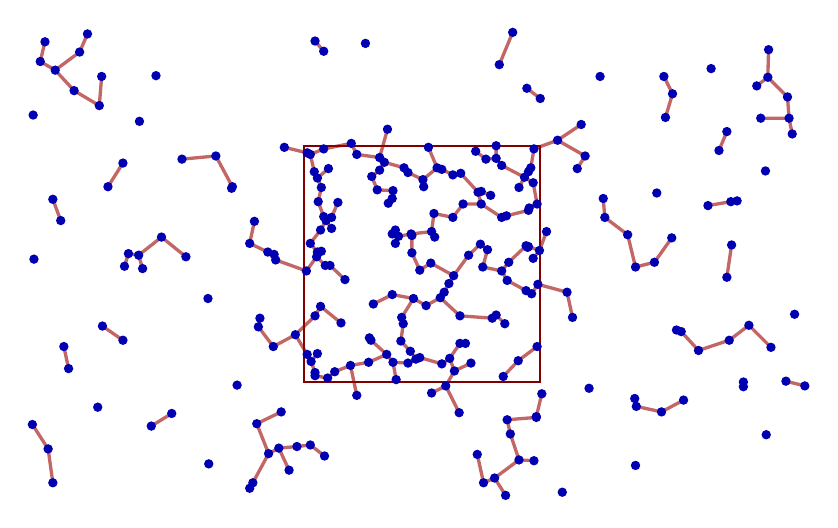
\begin{tikzpicture}[>=stealth]
    \tikzset{dot/.style={circle, fill=blue!70!black, inner sep=1.2pt, outer sep=0pt}}
    \tikzset{edge/.style={line width=1.2pt, red!60!black, opacity=0.6}}
    \tikzset{sq/.style={thick, red!50!black}}

    \draw[sq] (3.5, 1.5) rectangle (6.5, 4.5);
      \draw[edge] (3.75,5.70)--(3.64,5.83) (7.32,3.59)--(7.30,3.83) (7.32,3.59)--(7.61,3.37) (1.56,0.94)--(1.82,1.10) (0.58,5.20)--(0.34,5.46) (0.58,5.20)--(0.90,5.01) (6.01,4.25)--(5.94,4.34) (6.01,4.25)--(6.30,4.10) (0.21,5.82)--(0.15,5.57) (8.32,1.27)--(8.04,1.12) (3.04,3.15)--(3.12,3.12) (3.04,3.15)--(2.81,3.26) (4.32,1.75)--(4.09,1.71) (4.32,1.75)--(4.55,1.85) (6.12,0.84)--(6.08,1.02) (6.12,0.84)--(6.23,0.51) (2.92,2.20)--(3.11,1.95) (2.92,2.20)--(2.94,2.31) (4.56,4.71)--(4.46,4.35) (2.00,3.09)--(1.69,3.34) (5.92,0.28)--(6.06,0.06) (5.92,0.28)--(5.78,0.22) (5.92,0.28)--(6.23,0.51) (6.08,1.02)--(6.45,1.05) (0.65,5.69)--(0.34,5.46) (0.65,5.69)--(0.75,5.92) (9.66,4.85)--(9.70,4.65) (9.66,4.85)--(9.30,4.85) (9.66,4.85)--(9.64,5.12) (3.05,0.59)--(2.90,0.97) (3.05,0.59)--(3.18,0.66) (3.05,0.59)--(2.85,0.22) (6.84,2.64)--(6.91,2.32) (6.84,2.64)--(6.47,2.74) (1.22,2.97)--(1.27,3.13) (0.34,5.46)--(0.15,5.57) (2.59,3.98)--(2.38,4.37) (2.59,3.98)--(2.58,3.96) (3.12,3.12)--(3.14,3.05) (5.47,1.11)--(5.30,1.45) (9.39,5.37)--(9.25,5.26) (9.39,5.37)--(9.40,5.72) (9.39,5.37)--(9.64,5.12) (5.98,5.53)--(6.15,5.94) (0.45,1.95)--(0.51,1.67) (3.89,1.63)--(4.09,1.71) (3.89,1.63)--(3.80,1.55) (8.29,2.14)--(8.51,1.90) (8.29,2.14)--(8.23,2.16) (2.81,3.26)--(2.87,3.54);
      \draw[edge] (7.72,1.19)--(8.04,1.12) (7.72,1.19)--(7.70,1.29) (7.07,4.37)--(6.72,4.57) (7.07,4.37)--(6.97,4.21) (3.58,0.70)--(3.41,0.68) (3.58,0.70)--(3.76,0.56) (8.63,3.74)--(8.92,3.79) (3.31,0.38)--(3.18,0.66) (3.11,1.95)--(3.39,2.10) (8.87,2.83)--(8.93,3.24) (1.20,4.28)--(1.01,3.98) (7.61,3.37)--(7.71,2.96) (7.71,2.96)--(7.95,3.02) (5.23,2.57)--(5.05,2.47) (5.23,2.57)--(5.48,2.34) (5.23,2.57)--(5.28,2.64) (0.25,0.65)--(0.05,0.96) (0.25,0.65)--(0.31,0.22) (0.31,3.82)--(0.41,3.55) (3.14,3.05)--(3.53,2.91) (9.08,1.50)--(9.08,1.44) (4.10,4.53)--(3.75,4.46) (4.10,4.53)--(4.17,4.39) (2.90,0.97)--(3.21,1.12) (6.33,5.23)--(6.50,5.10) (8.07,5.38)--(8.18,5.16) (3.18,0.66)--(3.41,0.68) (8.18,5.16)--(8.09,4.86) (4.17,1.33)--(4.09,1.71) (1.20,2.03)--(0.94,2.21) (9.43,1.94)--(9.15,2.22) (5.19,4.22)--(5.01,4.07) (5.19,4.22)--(5.08,4.48) (5.19,4.22)--(5.25,4.20) (9.62,1.51)--(9.86,1.45) (4.97,1.81)--(4.92,1.79) (4.97,1.81)--(5.25,1.73) (2.85,0.22)--(2.81,0.15) (6.10,3.02)--(6.32,3.23) (6.10,3.02)--(6.01,2.91) (1.45,2.94)--(1.40,3.11) (6.72,4.57)--(7.02,4.77) (6.72,4.57)--(6.42,4.46) (2.38,4.37)--(1.95,4.33) (3.68,3.79)--(3.75,3.60) (3.68,3.79)--(3.72,3.97) (6.34,3.21)--(6.32,3.23) (6.34,3.21)--(6.35,3.22) (0.90,5.01)--(0.93,5.38) (5.12,1.36)--(5.30,1.45);
      \draw[edge] (6.45,1.05)--(6.45,1.06) (8.17,3.33)--(7.95,3.02) (5.30,1.45)--(5.41,1.64) (9.00,3.80)--(8.92,3.79) (3.39,2.10)--(3.54,1.85) (3.39,2.10)--(3.64,2.34) (8.87,4.68)--(8.77,4.44) (6.42,0.50)--(6.23,0.51) (5.49,4.15)--(5.39,4.13) (5.49,4.15)--(5.71,3.91) (6.52,1.35)--(6.45,1.06) (3.25,4.48)--(3.54,4.41) (6.58,3.41)--(6.49,3.17) (5.77,2.96)--(5.83,3.18) (5.77,2.96)--(6.01,2.91) (9.15,2.22)--(8.90,2.03) (8.51,1.90)--(8.90,2.03) (1.69,3.34)--(1.40,3.11) (5.70,0.58)--(5.78,0.22) (1.40,3.11)--(1.27,3.13) (3.59,1.76)--(3.54,1.85) (3.59,1.76)--(3.64,1.62) (3.59,1.76)--(3.67,1.86) (5.11,3.01)--(4.97,2.92) (5.11,3.01)--(5.40,2.85) (4.66,3.26)--(4.70,3.35) (3.66,3.09)--(3.77,2.98) (3.66,3.09)--(3.67,3.15) (3.66,3.09)--(3.53,2.91) (5.12,3.41)--(5.15,3.64) (5.12,3.41)--(5.16,3.34) (5.12,3.41)--(4.86,3.38) (5.68,4.43)--(5.81,4.33) (5.05,2.47)--(4.89,2.56) (5.89,2.31)--(5.48,2.34) (5.89,2.31)--(5.94,2.35) (4.82,1.74)--(4.92,1.79) (4.82,1.74)--(4.63,1.75) (3.58,4.39)--(3.75,4.46) (3.58,4.39)--(3.54,4.41) (3.58,4.39)--(3.63,4.17) (6.01,3.59)--(6.07,3.61) (6.01,3.59)--(5.75,3.76) (4.73,2.02)--(4.76,2.24) (4.73,2.02)--(4.85,1.89) (3.97,2.25)--(3.71,2.46) (5.15,3.64)--(5.39,3.59) (6.36,3.71)--(6.46,3.76) (6.36,3.71)--(6.35,3.68) (4.76,2.24)--(4.74,2.32);
      \draw[edge] (4.57,3.77)--(4.62,3.83) (3.64,1.62)--(3.64,1.58) (6.07,3.61)--(6.35,3.68) (4.92,1.79)--(4.85,1.89) (4.97,2.92)--(4.87,3.14) (4.02,2.80)--(3.83,2.98) (4.70,3.35)--(4.62,3.38) (4.70,3.35)--(4.86,3.38) (5.41,1.64)--(5.35,1.80) (5.41,1.64)--(5.62,1.74) (4.62,3.38)--(4.66,3.43) (5.01,4.07)--(5.02,3.98) (5.01,4.07)--(4.82,4.16) (5.48,1.99)--(5.35,1.80) (5.48,1.99)--(5.55,1.99) (3.71,3.43)--(3.58,3.26) (3.71,3.43)--(3.78,3.55) (3.58,3.26)--(3.67,3.15) (4.87,3.14)--(4.87,3.36) (6.32,2.66)--(6.08,2.79) (6.32,2.66)--(6.39,2.62) (6.38,4.22)--(6.35,4.17) (6.38,4.22)--(6.42,4.46) (3.80,1.55)--(3.64,1.58) (3.78,3.55)--(3.85,3.59) (3.78,3.55)--(3.75,3.60) (3.78,3.55)--(3.85,3.45) (3.71,2.46)--(3.64,2.34) (6.03,1.57)--(6.22,1.77) (5.94,2.35)--(6.05,2.24) (3.85,3.59)--(3.93,3.78) (5.39,4.13)--(5.25,4.20) (5.71,3.91)--(5.75,3.92) (5.71,3.91)--(5.75,3.76) (4.35,2.03)--(4.55,1.85) (4.35,2.03)--(4.33,2.06) (5.75,3.92)--(5.87,3.87) (6.47,2.74)--(6.39,2.62) (4.62,3.83)--(4.63,3.93) (4.52,4.29)--(4.46,4.19) (4.52,4.29)--(4.46,4.35) (4.52,4.29)--(4.77,4.22) (6.08,2.79)--(6.01,2.91) (5.75,3.76)--(5.52,3.76) (3.81,4.21)--(3.67,4.09) (4.46,4.19)--(4.36,4.11) (4.67,1.53)--(4.63,1.75) (6.22,1.77)--(6.46,1.95) (4.46,4.35)--(4.17,4.39) (6.35,3.22)--(6.49,3.17);
      \draw[edge] (5.40,2.85)--(5.59,3.11) (5.40,2.85)--(5.34,2.75) (4.38,2.49)--(4.62,2.61) (5.52,3.76)--(5.39,3.59) (3.77,2.98)--(3.83,2.98) (3.67,3.15)--(3.72,3.16) (4.82,4.16)--(4.77,4.22) (4.55,1.85)--(4.63,1.75) (5.35,1.80)--(5.25,1.73) (3.72,3.97)--(3.67,4.09) (4.62,2.61)--(4.89,2.56) (5.94,4.34)--(5.94,4.50) (5.94,4.34)--(5.81,4.33) (6.46,3.76)--(6.41,4.03) (5.83,3.18)--(5.74,3.25) (5.74,3.25)--(5.59,3.11) (4.36,4.11)--(4.43,3.94) (3.63,4.17)--(3.67,4.09) (6.41,3.07)--(6.49,3.17) (4.86,3.38)--(4.87,3.36) (6.35,4.17)--(6.30,4.10) (4.89,2.56)--(4.74,2.32) (4.43,3.94)--(4.63,3.93) (6.23,3.97)--(6.30,4.10) (5.34,2.75)--(5.28,2.64) (6.30,4.10)--(6.41,4.03);
    \foreach \x/\y in {3.75/5.70, 7.32/3.59, 1.56/0.94, 0.58/5.20, 6.01/4.25, 0.21/5.82, 8.32/1.27, 1.82/1.10, 3.04/3.15, 4.32/1.75, 6.12/0.84, 2.92/2.20, 4.56/4.71, 2.00/3.09, 5.92/0.28, 6.08/1.02, 0.65/5.69, 9.66/4.85, 3.05/0.59, 6.84/2.64, 1.22/2.97, 0.34/5.46, 2.59/3.98, 3.12/3.12, 5.47/1.11, 9.70/4.65, 9.39/5.37, 5.98/5.53, 0.88/1.18, 0.45/1.95, 3.89/1.63, 8.29/2.14, 2.81/3.26, 1.41/4.81, 0.75/5.92, 7.72/1.19, 0.06/4.89, 7.07/4.37, 7.71/0.44, 3.58/0.70, 8.63/3.74, 3.31/0.38, 3.11/1.95, 7.30/3.83, 8.87/2.83, 1.20/4.28, 7.61/3.37, 7.71/2.96, 5.23/2.57, 0.25/0.65, 0.31/3.82, 3.14/3.05, 9.08/1.50, 4.10/4.53, 2.29/0.46, 2.90/0.97, 9.30/4.85, 6.33/5.23, 8.04/1.12, 8.93/3.24, 8.07/5.38, 3.18/0.66, 2.28/2.56, 8.18/5.16, 0.07/3.06, 4.17/1.33, 1.20/2.03, 9.43/1.94, 5.19/4.22, 3.64/5.83, 9.62/1.51, 4.97/1.81, 2.85/0.22, 6.10/3.02, 0.51/1.67, 9.08/1.44, 1.45/2.94, 9.86/1.45, 6.72/4.57, 2.38/4.37, 3.68/3.79, 6.34/3.21, 0.90/5.01, 3.21/1.12, 0.41/3.55, 6.78/0.10, 5.12/1.36, 6.45/1.05, 6.91/2.32, 9.37/0.83, 3.41/0.68, 9.25/5.26, 2.58/3.96, 8.17/3.33, 5.30/1.45, 0.93/5.38, 9.00/3.80, 3.39/2.10, 7.26/5.38, 8.87/4.68, 6.42/0.50, 1.62/5.39, 6.06/0.06, 1.01/3.98, 0.05/0.96, 5.49/4.15, 6.52/1.35, 7.12/1.42, 3.25/4.48, 6.50/5.10, 6.58/3.41, 0.94/2.21, 2.65/1.46, 9.73/2.36, 8.92/3.79, 7.95/3.02, 5.77/2.96, 1.95/4.33, 2.81/0.15, 6.45/1.06, 9.40/5.72, 9.15/2.22, 0.15/5.57, 4.28/5.80, 9.64/5.12, 2.94/2.31, 8.51/1.90, 1.69/3.34, 9.36/4.18, 5.70/0.58, 6.15/5.94, 1.40/3.11, 8.77/4.44, 6.97/4.21, 3.59/1.76, 8.09/4.86, 8.67/5.48, 5.11/3.01, 7.98/3.90, 7.02/4.77, 8.90/2.03, 3.76/0.56, 5.78/0.22, 4.66/3.26, 2.87/3.54, 0.31/0.22, 8.23/2.16, 1.27/3.13, 7.70/1.29, 6.23/0.51, 3.66/3.09, 5.12/3.41, 5.68/4.43, 5.05/2.47, 5.89/2.31, 4.82/1.74, 3.58/4.39, 6.01/3.59, 4.73/2.02, 3.97/2.25, 5.15/3.64, 5.48/2.34, 6.36/3.71, 5.16/3.34, 4.76/2.24, 4.57/3.77, 3.54/1.85, 3.64/1.62, 6.07/3.61, 4.92/1.79, 4.97/2.92, 4.02/2.80, 4.70/3.35, 5.41/1.64, 4.62/3.38, 5.01/4.07, 5.48/1.99, 3.71/3.43, 3.58/3.26, 6.32/3.23, 4.66/3.43, 4.87/3.14, 6.32/2.66, 6.38/4.22, 4.09/1.71, 3.80/1.55, 3.78/3.55, 3.71/2.46, 6.03/1.57, 5.94/2.35, 3.85/3.59, 5.39/4.13, 5.71/3.91, 4.35/2.03, 5.75/3.92, 6.47/2.74, 4.62/3.83, 4.52/4.29, 6.08/2.79, 5.75/3.76, 3.81/4.21, 5.02/3.98, 4.46/4.19, 4.67/1.53, 6.22/1.77, 4.46/4.35, 6.35/3.22, 5.40/2.85, 4.38/2.49, 5.52/3.76, 5.87/3.87, 3.77/2.98, 3.67/3.15, 4.82/4.16, 4.55/1.85, 3.93/3.78, 5.35/1.80, 3.75/3.60, 3.72/3.97, 5.62/1.74, 3.75/4.46, 4.62/2.61, 5.94/4.34, 6.46/3.76, 4.63/1.75, 5.83/3.18, 4.77/4.22, 3.83/2.98, 3.53/2.91, 3.67/1.86, 3.85/3.45, 5.74/3.25, 6.39/2.62, 4.36/4.11, 4.17/4.39, 3.54/4.41, 3.63/4.17, 5.08/4.48, 3.72/3.16, 6.41/3.07, 5.39/3.59, 4.86/3.38, 5.25/4.20, 3.64/2.34, 6.35/4.17, 4.87/3.36, 4.33/2.06, 4.89/2.56, 5.25/1.73, 6.42/4.46, 5.59/3.11, 4.43/3.94, 5.55/1.99, 6.23/3.97, 6.35/3.68, 5.34/2.75, 6.30/4.10, 3.64/1.58, 4.63/3.93, 6.46/1.95, 5.28/2.64, 6.41/4.03, 6.01/2.91, 4.74/2.32, 3.67/4.09, 5.94/4.50, 6.49/3.17, 5.81/4.33, 6.05/2.24, 4.85/1.89} {
        \node[dot] at (\x, \y) {};
    }
  \end{tikzpicture}
  }
  \caption{Arbre minimum couvrant élagué à $r$.}
  \label{fig:mst}
\end{subfigure}

  \caption{Illustration du \Th~\ref{th:mst_gg} : le graphe géométrique (à gauche) et l'arbre minimum couvrant élagué au même rayon (à droite) partagent rigoureusement les mêmes composantes connexes.\label{fig:MST_GrapheGeometrique}}
\end{figure}





% \begin{figure}[!ht]
% \begin{center}
%     \begin{tikzpicture}[scale=0.9]
%         \fill[blue!10] (0,0) ellipse (1.8 and 1.2);
%         \node[blue!80!black] at (-0.5, 0.5) {$\mathcal{X}_1$};
%         \fill (1, 0) circle (2pt) node[below] {$x_1$};
        
%         \fill[red!10] (5,0) ellipse (1.5 and 1.2);
%         \node[red!80!black] at (5.5, 0.5) {$\mathcal{X}_2$};
%         \fill (4, 0.2) circle (2pt) node[below] {$x_2$};
        
%         \draw[thick, dashed] (1, 0) -- (4, 0.2) node[midway, above] {$2r_{\mathrm{connect}}$};
%     \end{tikzpicture}
% \end{center}
% \caption{Pour $r \lesssim r_{\mathrm{connect}}$, le graphe géométrique $\mathcal{G}(\mathcal X, r)$ se sépare en deux composantes connexes $\mathcal X_1$ et $\mathcal X_2$.}
% \label{fig:r_connect}
% \end{figure}

Ce résultat est précieux car il relie intimement le Single-Linkage à la théorie de la percolation continue \cite{MeesterRoy, penrose2003, BibiIstambul}. Nous reviendrons sur ce mécanisme, la percolation, au cœur du Single-Linkage et de tous les algorithmes de la même famille au chapitre \ref{sec:chap_percolation}.


Utilisé dans l'autre sens (si l'on souhaite construire le clustering produit par le Single-Linkage pour un petit seuil $\eps$), le \Th~\ref{th:mst_gg} montre qu'il suffit d'identifier les composantes connexes du ``petit'' graphe géométrique de rayon $r \gets \eps$ ; il n'y a pas besoin de reconstruire tout l'arbre minimum couvrant.

\section{Le modèle statistique du Single-Linkage : \nom{Hartigan} et les amas de forte densité}


\subsection{Amas de forte densité (\emph{high-density clusters})}

C'est sous l'impulsion de \nom{Hartigan} \cite{hartigan75} que le clustering hiérarchique a trouvé un ancrage mathématique rigoureux. Plutôt que de voir le clustering comme une simple heuristique de graphes, on suppose que les données $\mathcal X \subset \mathbb R^p$ sont des réalisations indépendantes issues d'une certaine densité par rapport à la mesure de \textsc{Lebesgue} 
\[
f : \mathbb R^p \to \mathbb R_+ .
\]

\begin{Definition}{Amas de forte densité, modèle de \nom{Hartigan} \cite{hartigan75}}{high-density_clusters}
Soit $\lambda > 0$. Commençons par définir l'ensemble de niveau supérieur à $\lambda$ pour la fonction $f$ :
\[
    L(\lambda) \eqdef \bigl\{ x \in \mathbb R^p   \bigm|   f(x) \ge \lambda \bigr\}.
\]

Les amas de forte densité (\emph{high-density clusters} en anglais) $H_f(\lambda)$ de la densité $f$ au niveau $\lambda$ sont définis comme les composantes connexes de $L(\lambda)$
\[
\boxed{
H_f(\lambda) \eqdef \pi_0 \big( H_f(\lambda)\bigr).
}
\]
\end{Definition}

En faisant varier $\lambda$, on observe une hiérarchie stricte d'amas s'emboîtant les uns dans les autres, formalisant mathématiquement le clustering sous forme d'un arbre hiérarchique continu (voir \Fig~\ref{fig:hartigan}). %En intersectant ces ensembles continus avec l'échantillon de données, on obtient les clusters discrets. % : $A_\lambda^{\mathrm{discr}} = A_\lambda \cap \mathcal X$.


\begin{figure}[!ht]
    \centering
    \begin{tikzpicture}[scale=0.8, >=latex, font=\small]
        % Paramètres des pics
        \def\xone{1.5} \def\hone{2.8}
        \def\xtwo{5.5} \def\htwo{2.0}
        \def\xsaddle{3.5} \def\hsaddle{0.8}
        \def\hlambda{1.3}

        % --- PARTIE HAUTE : DENSITÉ f(x) ---
        \begin{scope}[yshift=4.2cm]
            \draw[->, thick] (0,-0.1) -- (0,3.2) node[left] {$f(x)$};
            \draw[->, thick] (-0.2,0) -- (7.5,0);
            
            % On nomme la courbe "curve" pour pouvoir calculer les intersections
            \draw[thick, blue!80!black, name path=curve] plot [smooth, tension=0.7] coordinates {
                (0,0.1) (\xone,\hone) (\xsaddle,\hsaddle) (\xtwo,\htwo) (7,0.1)
            };
            
            % On nomme la droite "line"
            \draw[dashed, red, thick, name path=line] (0,\hlambda) -- (7,\hlambda) node[right] {$\lambda$};
            
            \begin{scope}
                \clip (0,\hlambda) rectangle (7,3.2);
                \fill[blue!20, opacity=0.6] plot [smooth, tension=0.7] coordinates {
                    (0,0.1) (\xone,\hone) (\xsaddle,\hsaddle) (\xtwo,\htwo) (7,0.1)
                } |- (0,0);
            \end{scope}

            % --- NOUVEAU : Intervalles A_\lambda et B_\lambda sur l'axe des abscisses ---
            % TikZ trouve les 4 points d'intersection (de gauche à droite)
            \path [name intersections={of=curve and line, by={i1,i2,i3,i4}}];
            
            % On trace les segments sur l'axe (y=0) grâce à la projection orthogonale " |- 0,0 "
            \draw[very thick, red] (i1 |- 0,0) -- (i2 |- 0,0) node[midway, below=2pt, font=\bfseries] {$A_\lambda$};
            \draw[very thick, red] (i3 |- 0,0) -- (i4 |- 0,0) node[midway, below=2pt, font=\bfseries] {$B_\lambda$};
            
            % Ajout de lignes de projection et de petits taquets verticaux pour délimiter les intervalles
            \foreach \k in {1,2,3,4} {
                % Ligne de projection en pointillés
                \draw[red!50, densely dotted, thin] (i\k) -- (i\k |- 0,0);
                % Taquet vertical façon crochet " [ ] "
                \draw[thick, red] (i\k |- 0,-0.1) -- (i\k |- 0,0.1);
            }
            % -----------------------------------------------------------------------------
            
            \fill[blue!80!black] (\xone,\hone) circle (1.5pt);
            \fill[blue!80!black] (\xtwo,\htwo) circle (1.5pt);
        \end{scope}

        % --- PARTIE BASSE : ARBRE HIÉRARCHIQUE ---
        \begin{scope}[yshift=0cm]
            \draw[->, thick] (0,0) -- (0,3.2) node[left] {$\lambda$};
            \draw[dashed, red, thick] (0,\hlambda) -- (7,\hlambda);

            \draw[very thick, black] (\xsaddle, 0) -- (\xsaddle, \hsaddle);
            \draw[very thick, black] (\xone, \hsaddle) -- (\xtwo, \hsaddle);
            \fill[gray] (\xsaddle, \hsaddle) circle (3.5pt);
            
            \draw[very thick, black] (\xone, \hsaddle) -- (\xone, \hone);
            \draw[very thick, black] (\xtwo, \hsaddle) -- (\xtwo, \htwo);
            
            \fill[white, draw=red, thick] (\xone, \hlambda) circle (2.5pt);
            \node[red, font=\bfseries, xshift=-12pt, yshift=-8pt] at (\xone, \hlambda) {$A_\lambda$};

            \fill[white, draw=red, thick] (\xtwo, \hlambda) circle (2.5pt);
            \node[red, font=\bfseries, xshift=12pt, yshift=-8pt] at (\xtwo, \hlambda) {$B_\lambda$};
            
            \draw[dotted, gray] (0, \hone) -- (\xone, \hone);
            \draw[dotted, gray] (0, \htwo) -- (\xtwo, \htwo);
            
            \draw[dotted, blue!50] (\xone, 4.2) -- (\xone, \hone);
            \draw[dotted, blue!50] (\xtwo, 4.2) -- (\xtwo, \htwo);
            \draw[dotted, blue!50] (\xsaddle, 4.2) -- (\xsaddle, \hsaddle);
        \end{scope}
    \end{tikzpicture}
    \caption{Le modèle de \nom{Hartigan} : correspondance entre $H_f(\lambda)$, les composantes connexes des ensembles de niveau de la densité $L(\lambda)$, (en haut) et la topologie de l'arbre hiérarchique des amas de forte densité (en bas).}
    \label{fig:hartigan}
\end{figure}


% \begin{figure}[!ht]
%     \centering
%     \begin{tikzpicture}[scale=0.8, >=latex, font=\small]
%         % Paramètres des pics
%         \def\xone{1.5} \def\hone{2.8}
%         \def\xtwo{5.5} \def\htwo{2.0}
%         \def\xsaddle{3.5} \def\hsaddle{0.8}
%         \def\hlambda{1.3}

%         % --- PARTIE HAUTE : DENSITÉ f(x) ---
%         \begin{scope}[yshift=4.2cm]
%             \draw[->, thick] (0,-0.1) -- (0,3.2) node[left] {$f(x)$};
%             \draw[->, thick] (-0.2,0) -- (7.5,0);
            
%             \draw[thick, blue!80!black] plot [smooth, tension=0.7] coordinates {
%                 (0,0.1) (\xone,\hone) (\xsaddle,\hsaddle) (\xtwo,\htwo) (7,0.1)
%             };
            
%             \draw[dashed, red, thick] (0,\hlambda) -- (7,\hlambda) node[right] {$\lambda$};
            
%             \begin{scope}
%                 \clip (0,\hlambda) rectangle (7,3.2);
%                 \fill[blue!20, opacity=0.6] plot [smooth, tension=0.7] coordinates {
%                     (0,0.1) (\xone,\hone) (\xsaddle,\hsaddle) (\xtwo,\htwo) (7,0.1)
%                 } |- (0,0);
%             \end{scope}
            
%             \fill[blue!80!black] (\xone,\hone) circle (1.5pt);
%             \fill[blue!80!black] (\xtwo,\htwo) circle (1.5pt);
%         \end{scope}

%         % --- PARTIE BASSE : ARBRE HIÉRARCHIQUE ---
%         \begin{scope}[yshift=0cm]
%             \draw[->, thick] (0,0) -- (0,3.2) node[left] {$\lambda$};
%             \draw[dashed, red, thick] (0,\hlambda) -- (7,\hlambda);

%             \draw[very thick, black] (\xsaddle, 0) -- (\xsaddle, \hsaddle);
%             \draw[very thick, black] (\xone, \hsaddle) -- (\xtwo, \hsaddle);
%             \fill[gray] (\xsaddle, \hsaddle) circle (3.5pt);
            
%             \draw[very thick, black] (\xone, \hsaddle) -- (\xone, \hone);
%             \draw[very thick, black] (\xtwo, \hsaddle) -- (\xtwo, \htwo);
            
%             % \fill[white, draw=red, thick] (\xone, \hlambda) circle (2.5pt);
%             % \node[red, left=8pt, below=2pt, font=\bfseries] at (\xone, \hlambda) {$A_\lambda$};
            
%             % \fill[white, draw=red, thick] (\xtwo, \hlambda) circle (2.5pt);
%             % \node[red, right=8pt, below=2pt, font=\bfseries] at (\xtwo, \hlambda) {$B_\lambda$};
%             \fill[white, draw=red, thick] (\xone, \hlambda) circle (2.5pt);
%             \node[red, font=\bfseries, xshift=-12pt, yshift=-8pt] at (\xone, \hlambda) {$A_\lambda$};

%             \fill[white, draw=red, thick] (\xtwo, \hlambda) circle (2.5pt);
%             \node[red, font=\bfseries, xshift=12pt, yshift=-8pt] at (\xtwo, \hlambda) {$B_\lambda$};
            
%             \draw[dotted, gray] (0, \hone) -- (\xone, \hone);
%             \draw[dotted, gray] (0, \htwo) -- (\xtwo, \htwo);
            
%             \draw[dotted, blue!50] (\xone, 4.2) -- (\xone, \hone);
%             \draw[dotted, blue!50] (\xtwo, 4.2) -- (\xtwo, \htwo);
%             \draw[dotted, blue!50] (\xsaddle, 4.2) -- (\xsaddle, \hsaddle);
%         \end{scope}
%     \end{tikzpicture}
%     \caption{Le modèle de \nom{Hartigan} : correspondance entre les composantes connexes des ensembles de niveau de la densité $H_f(\lambda)$ (en haut) et la topologie de l'arbre hiérarchique des amas de forte densité (en bas).}
%     \label{fig:hartigan}
% \end{figure}


\subsection{L'estimateur de densité des $K$-Plus Proches Voisins ($K$-NN)}

En pratique, la densité $f$ est inconnue ; l'approche statistique classique consiste à en construire un estimateur $\widehat f$.
L'estimateur des $K$-Plus Proches Voisins ($K$-NN pour $K$-\emph{Nearest Neighbours} en anglais) \cite{BiauDevroye} est le choix non-paramétrique le plus naturel pour ce faire.

\begin{Definition}{Estimateur de densité des $K$-Plus Proches Voisins ($K$-NN) \cite{BiauDevroye}}{K-NN}
Soit $\mathcal X \subset \mathbb R^p $ un nuage de l'espace euclidien contenant $n\in \mathbb N^\star$ points et $K \in \mathbb N^\star$ un entier avec tel que $K \le n$. L'estimateur de densité des $K$-Plus Proches Voisins $\widehat f_{K}$ (noté plus simplement $\widehat \lambda$) est défini pour tout point $y \in \mathbb R^p$ par 
\[
\boxed{
    \widehat \lambda = \widehat f_{K}(y) \eqdef \frac{K}{n}  \frac{1}{\omega_p r_K(y)^p} 
}
\]
où $r_K(y) = \inf \bigl\{ r \ge 0 \bigm| \module{B(y, r) \cap \mathcal X} \ge K \bigr\}$ représente la distance de $y$ à son $K$-ième plus proche voisin, et $\omega_p$ le volume de la boule unité dans $\mathbb R^p$.

On définit aussi les niveaux supérieurs associés à cet estimateur pour $\lambda > 0$
\[
    L_K(\lambda) \eqdef \bigl\{ y \in \mathbb R^p \bigm|  \widehat f_K(y) \ge \lambda \bigr\}.
\]
\end{Definition}
\Remarques{
\begin{enumerate}
    \item Dans le cas particulier $K=1$ et $y \in \mathcal X$, on pose $\widehat f_1(y) = +\infty$.
    \item Au facteur $\frac{K}{n}$ de normalisation près, $\widehat \lambda$ est l'inverse du volume de la plus petite boule centrée en $y$ englobant $K$ points de $\mathcal X$.
    \item La condition d'être au-dessus d'un certain seuil de densité estimée, $\hat f_{K}(y) \ge \lambda$, est strictement équivalente à se trouver à une distance $r_K(y) \le r$ d'un point du nuage, avec le changement de variable 
    \[
        \lambda = \frac{K}{n \, \omega_p \,  r^p}.
    \]
    Dans la suite, on manipulera indifféremment les variables $\lambda$ ou $r$, étant sous-entendu ce changement de variable.
\end{enumerate}}




\subsection{Lien entre le Single-Linkage et la hiérarchie de \textsc{Hartigan} $1$-NN}
\label{sec:lien_SL_HartiganNN}

Le lien fondamental avec le Single-Linkage apparaît dans le cas très particulier où $K=1$ : l'ensemble de niveau se réduit alors au \emph{modèle booléen} d'union de boules \cite{MeesterRoy} :
\[
    L_1(r) \eqdef \bigl\{ y \in \mathbb R^p \bigm| r_1(y) \le r \bigr\} = \bigcup_{x \in \mathcal X} \overline{B}(x, r).
\]

Les composantes connexes de cette union de boules correspondent aux composantes connexes du graphe géométrique $\mathcal G(\mathcal X, r)$ qui sont elles-mêmes en correspondance avec l'arbre minimum couvrant élagué à $r$ (d'après le \Th~\ref{th:mst_gg}).
\emph{Confer} la synthèse en fin de chapitre.


\subsection{Amas de forte densité \emph{discrets}}

Pour tout entier $K \le n$, on dispose d'un estimateur de densité $\widehat f_{K} \colon \mathbb R^p \to \mathbb R_+$.
%Appliquer la définition des amas de forte densité (\Def~\ref{def:high-density_clusters}) $H_f(\cdot)$ directement en remplaçant $f \gets \widehat f_{K}$ $f$ produit un arbre hiérarchique 
Appliquer directement la définition des amas de forte densité (\Def[def:high-density_clusters]) pour construire $H_f(\cdot)$  en assignant $f \gets \widehat f_{K}$ produit un arbre hiérarchique dont les éléments sont des sous-ensembles de $\mathbb R^p$ ; l'on souhaiterait des sous-ensembles de nos données $\mathcal X$. Introduisons pour cela la notion d'amas de forte densité \emph{discret}.

\begin{Definition}{Amas de forte densité discrets}{HDC_discret}
Soit $\mathcal X \subset \mathbb R^p$ un nuage fini de taille $n$ et $K \le n$ un entier. 
Soit $\widehat f_K$ l'estimateur de densité $K$-NN associé et 
\[
H_{\widehat f_K} \colon r > 0\mapsto \pi_0\left( L_K(r)\right)
\]
les amas de forte densité de $f_K$, c'est-à-dire la fonction qui à un niveau $r > 0$ associe les composantes du niveau supérieur $L_K(r)$.

L'on dira que $x \in \mathcal X$ est \emph{couvert} par un certain cluster  $C \in H_{\widehat f_K}(r)$ s'il se trouve à moins de $r$ de ce même cluster. Le cluster $C^{\mathrm{discret}}$ associé à $C$ est alors l'ensemble des points $x\in \mathcal X$ qui sont couverts par $C$.
Finalement, on définit les amas de forte densité \emph{discrets} pour $f_K$ au niveau $r > 0$ par
\[
\boxed{
     H_{\widehat f_K}^{\mathrm{discrets}}(r) \eqdef  \left\{ C^{\mathrm{discret}} \bigm|  C \in  H_{\widehat f_K}(r)  \right\}.
    }
\]
\end{Definition}

\Remarques{
\begin{enumerate}
    \item L'idée derrière cette définition de $C^{\mathrm{discret}}$ est de bien prendre en compte tous les points qui participent à la formation de l'amas de forte densité associé. Poser $C^{\mathrm{discret}} = C \cap \mathcal X$ aurait été une erreur. (Erreur que l'on quantifiera exactement dans le chapitre \ref{sec:chap_percolation} consacré au phénomène de percolation.) Cette distinction est d'ailleurs la différence essentielle entre le Robust Single-Linkage et DBSCAN (voir \emph{infra} \Def[def:dbscan_points]) -- et qui explique d'ailleurs la supériorité de DBSCAN sur le Robust Single-Linkage.
    \item L'on a défini l'amas discret $C^{\mathrm{discret}}$ associé à $C \in H_{\widehat f_K}(r)$ comme l'ensemble des points $x \in \mathcal X$ à une distance de $C$ inférieure à $r$. Cela équivaut à poser
\[
        C^{{\mathrm{discret}}} = \mathcal X \cap \delta_r(C)
\]
    où $\delta_r(C)$ désigne la dilatation de l'ensemble $C$ de rayon $r$.
    \item Sauf dans le cas particulier $K=1$, les amas discrets de forte densité ne forment pas une partition de $\mathcal X$ ; pour un certain niveau $r > 0$ fixé, certains points $x \in \mathcal X$ peuvent n'être couverts par aucun cluster, d'autres points peuvent être couverts par plusieurs clusters.
\end{enumerate}
}




\Synthese{
Finalement, le clustering hiérarchique produit par l'algorithme du Single-Linkage peut être calculé de trois façons différentes.
Soit $t \in \bigl\{ 0 ; \ldots ; n-1 \bigr\}$ l'étape à laquelle on s'arrête et $r_t$ le rayon de coupure associé (voir \emph{supra} \Def[single-linkage]). Soit $\lambda_t = \frac{1}{n \, \omega_p \,  r_t^p}$ la variable de densité associée au rayon.
La partition $\mathcal C^{r_t}$ peut être obtenue de trois façons différentes :}
\begin{align*}
    \mathcal C^{r_t} &= \text{Composantes connexes du graphe géométrique } \mathcal{G}(\mathcal X, r_t) ; \\
                 &= \text{Composantes connexes de l'arbre minimum couvrant élagué } \mathrm{MST}_{\le r_t} ;\\
                 &= \text{Amas discrets de forte densité } H^{\mathrm{discrets}}_{\widehat f_{1}}(\lambda_t).
\end{align*}

Cette synthèse intègre le Single-Linkage dans la famille de clusterings \emph{density-based} \cite{DensityBasedClustering} et trace la voie naturelle pour sa généralisation aux estimateurs d'ordre supérieur avec $K \ge 2$.